\documentclass[12pt,a4paper]{report}

\usepackage[T1]{fontenc}
\usepackage[utf8]{inputenc}
\usepackage[margin=1in]{geometry}
\usepackage{setspace}
\usepackage{amsmath}
\usepackage{newtxtext,newtxmath}
\usepackage[round,authoryear]{natbib}
\usepackage{graphicx}
\usepackage{booktabs}
\usepackage{longtable}
\usepackage{array}
\usepackage{siunitx}
\usepackage[hidelinks]{hyperref}
\usepackage{caption}
\usepackage{subcaption}
\usepackage{float}
\usepackage{titlesec}
\usepackage{fancyhdr}
\usepackage{tikz}
\usepackage{pgfplots}
\pgfplotsset{compat=1.16}
\usetikzlibrary{arrows.meta,positioning,shapes.geometric,fit,backgrounds}
\graphicspath{{frontend/images/}}

\setcitestyle{authoryear,round}

% Research-paper style heading scale with separator rules.
\titleformat{\chapter}[display]
    {\normalfont\bfseries\Large}
    {\chaptertitlename\ \thechapter}{0.6em}{\Large}
    [\vspace{0.4em}\titlerule]
\titlespacing*{\chapter}{0pt}{-8pt}{14pt}
\titleformat{\section}{\normalfont\bfseries\large}{\thesection}{0.7em}{}
\titlespacing*{\section}{0pt}{10pt}{6pt}
\titleformat{\subsection}{\normalfont\bfseries\normalsize}{\thesubsection}{0.7em}{}
\titlespacing*{\subsection}{0pt}{8pt}{4pt}

\title{\textbf{Insurance Fraud Detection\\Using Hybrid Machine Learning Approaches:}\\
A Comparative Study of\\ML Algorithms and Statistical Methods}
\author{Ruslan Sheikh\\
BC\&DA Final Year Project}
\date{April 2026}

\begin{document}
\setstretch{1.18}
\setlength{\headheight}{15pt}
\pagestyle{fancy}
\fancyhf{}
\fancyhead[L]{\nouppercase{\leftmark}}
\fancyhead[R]{\thepage}
\renewcommand{\headrulewidth}{0.4pt}
\renewcommand{\footrulewidth}{0pt}

\pagenumbering{roman}
\maketitle

\chapter*{Abstract}
\addcontentsline{toc}{chapter}{Abstract}
Insurance fraud harms insurers in more ways than payout leakage alone. Review queues grow, settlement cycles slow, and trust in digital claims channels starts to weaken. For that reason, fraud detection is not only a modeling task; it is a decision-quality task.

This study asks whether a hybrid framework can improve both detection performance and operational usefulness under controlled conditions. The model combines three evidence channels: supervised machine learning (XGBoost), Benford-based statistical anomaly checks, and deterministic policy rules. Evaluation follows a strict sequence with shared partitions, fold-level calibration, and post-hoc robustness checks to keep comparisons fair.

Because production claim data was unavailable under privacy and governance constraints, the study used a synthetic pipeline with explicit realism validation at distributional, relational, and operational levels. The final dataset includes 1,200 claims with 18\% fraud prevalence and Hong Kong-aligned context. On a common holdout set, the hybrid model reached 92.0\% accuracy, 89.5\% precision, 88.2\% recall, and 88.8\% F1, outperforming ML-only (90.1\%), Benford-only (78.3\%), and rule-only (74.1\%).

The contribution is practical and methodological. The paper introduces a governance-oriented hybrid protocol, reports comparative and robustness evidence beyond headline metrics, and links model outputs to a web-based decision-support interface for claims operations.

The central finding is simple: metric gains matter only when they hold up under audit, stress, and real decision pressure. Framed this way, fraud analytics becomes a socio-technical design problem rather than a narrow classifier contest.

\chapter*{AI Usage Declaration}
\addcontentsline{toc}{chapter}{AI Usage Declaration}
Artificial intelligence tools were used in this project to synthesize the author's ideas into clearer written structure and to improve grammar and language quality. All technical decisions, analytical interpretations, and final research claims were reviewed and validated by the author.

\tableofcontents
\listoffigures
\listoftables

\chapter*{List of Abbreviations}
\addcontentsline{toc}{chapter}{List of Abbreviations}
\begin{longtable}{p{0.23\textwidth}p{0.70\textwidth}}
\toprule
\textbf{Abbreviation} & \textbf{Meaning} \\
\midrule
\endhead
AI & Artificial Intelligence \\
AUC-ROC & Area Under the Receiver Operating Characteristic Curve \\
CI & Confidence Interval \\
ECE & Expected Calibration Error \\
FPR & False Positive Rate \\
HK & Hong Kong \\
MCE & Maximum Calibration Error \\
ML & Machine Learning \\
RQ & Research Question \\
SMOTE & Synthetic Minority Over-sampling Technique \\
\bottomrule
\end{longtable}

\pagenumbering{arabic}

\chapter{Introduction}

\section{Research Background}
Insurance fraud imposes two distinct costs. One is direct and easy to count: illegitimate payouts. The other unfolds inside operations, where investigation queues expand, settlement slows, and confidence in digital claims handling begins to erode. Detection therefore has to do more than score well on paper; it must support timely action \citep{bolton2002,phua2010}.

In Hong Kong, this issue carries real financial weight. Insurance Authority figures indicate a large premium base, meaning even small leakage rates can scale into substantial portfolio losses \citep{ia2024}. Prior fraud studies also show that when controls remain static, abuse can absorb a non-trivial share of claims outflow \citep{caif2022}.

Medical claims rarely follow one neat risk pattern. Behavior differs by provider, policy age, and treatment type, so a detector that performs well in one pocket may underperform in another. ML methods capture richer interactions but are often harder to interpret. Statistical checks are easier to explain, yet narrower in scope. Rule systems are transparent, though they can go stale over time. Put plainly, no single lens sees the whole picture; a multi-signal design is the practical alternative \citep{chen2016,durtschi2004,subelj2011}.

With that context, this study does not ask which standalone model tops a leaderboard. It asks whether combining evidence can improve fraud capture, reduce avoidable review work, and remain explainable enough for governance.

\section{Economic and Operational Urgency}
The urgency is financial, but it is also deeply operational. Slow or poorly targeted detection lets losses accumulate while analysts burn time on weak leads. The result is a two-sided penalty: missed fraud and unnecessary manual effort.

This project addresses that mismatch directly. The aim is stronger decision quality through better case prioritization, clearer escalation rationale, and more consistent oversight. Accuracy still matters, of course, but in insurer operations it is only part of the decision equation.

\section{Research Purpose and Questions}
The study evaluates whether a weighted hybrid model can outperform standalone approaches without losing interpretability or workflow fit. Rather than ending at benchmark tables, it connects model behavior to triage and governance requirements.

Primary research question: \emph{Does a weighted hybrid model improve fraud detection outcomes over standalone ML, statistical, and rule-based baselines under identical evaluation constraints?} Supporting hypotheses examine whether recall and F1 improve, and whether those improvements remain operationally usable instead of generating excess false-positive burden.

A key concern sits behind that question: are gains structural, or are they artifacts of tuning and split luck? To answer that, the design includes ablation and uncertainty analysis alongside headline metrics.

\section{Statement of Novelty and Contribution Boundary}
The novelty claim is intentionally narrow. This paper does not claim that hybrid modeling is new by itself. It argues that a \textbf{governance-oriented hybrid protocol} can produce measurable uplift while staying interpretable under controlled constraints.

That contribution rests on three design choices: (1) strict evaluation discipline with locked splits and staged ablation, (2) explicit linkage between model evidence and operational decision surfaces, and (3) reporting that joins performance metrics with uncertainty, calibration, and utility framing.

The boundary is stated clearly. The output is a reproducible \emph{research-to-operations template} in a synthetic yet domain-aligned Hong Kong setting, not a universal generalization claim.

\section{Why This Study Is Needed}
Many fraud studies report better metrics without showing how those gains affect deployment decisions, particularly in regulated settings that demand explanation and audit traceability \citep{phua2010,bolton2002}. This work addresses that gap by treating predictive quality, explanation quality, and workflow impact as joint objectives.

The practical motivation is straightforward. Static thresholds and manual queues remain common in insurer operations because they are familiar and easy to justify, yet they adapt slowly. This study tests whether integrated detection can raise decision quality without compromising governance expectations.

\section{Scope}
This paper focuses on medical-claim fraud detection and evaluates methods on a synthetic, domain-aligned Hong Kong dataset. It is designed as a rigorous baseline study with deployment relevance, not as a direct production claim.

Validity is bounded at three levels: internal validity (fairness of comparison), construct validity (how well synthetic features represent fraud mechanisms), and external validity (the extent to which findings transfer to real claims). These limits are made explicit throughout the manuscript.

\chapter{Literature Review and Theoretical Foundation}

\section{Machine Learning Approaches for Fraud Detection}
Ensemble tree methods, especially gradient boosting, are widely used in tabular fraud modeling because they capture nonlinear interactions without relying on strict distributional assumptions \citep{chen2016}. In claims data, risk usually emerges from signal combinations rather than isolated variables. XGBoost performs well in this setting, but only when class imbalance and threshold calibration are handled with care \citep{chawla2002}.

The literature also makes one point repeatedly: evaluation discipline matters as much as model choice. Leakage-prone preprocessing, inconsistent split rules, or threshold tuning on holdout data can inflate reported gains. Evaluation, then, should be treated as experimental design rather than a scoreboard exercise.

Another consistent finding is that discrimination alone is insufficient in high-stakes settings. Intervention requires explainable evidence. For this reason, the present study treats ML as a strong core channel, but not as a standalone end-state.

\section{Statistical Detection Using Benford's Law}
Benford's Law is a standard forensic tool for detecting unusual numeric patterns, particularly where value manipulation is suspected \citep{benford1938,durtschi2004}. For leading digits, the expected probability is:
\begin{equation}
P(d) = \log_{10}\left(1 + \frac{1}{d}\right), \quad d \in \{1,\dots,9\}
\end{equation}
When observed first-digit frequencies deviate materially from this curve, the stream may warrant further review.

The method's main advantage is interpretability; non-technical stakeholders can understand the signal quickly. Its weakness is narrower coverage. Benford captures specific anomaly classes but does not model richer behavioral interactions, so it is better used as a complementary channel than as an ML substitute.

Prior work also warns that benign subgroup structure can produce Benford deviation \citep{durtschi2004}. That limitation supports using Benford as weighted evidence, not as a sole decision trigger.

\section{Rule-Based Systems and Domain Knowledge}
Rule-based systems remain common because they encode policy logic directly and are straightforward to audit \citep{subelj2011}. They are especially useful for high-confidence violations with clear institutional definitions. Their main weakness is adaptability, since static thresholds can lose effectiveness as fraud behavior shifts.

Rules also provide governance value beyond pure detection performance. They support traceability for compliance and management review. Replacing them entirely with opaque optimization may weaken institutional trust, even when short-run performance appears stronger.

\section{Hybrid Detection as a Research Direction}
Prior studies repeatedly show that mixed-method detection can outperform single-family models because fraud behavior is heterogeneous \citep{phua2010,yue2007}. In practical terms, hybridization diversifies evidence channels and reduces dependence on any one model.

Fusion, however, is not a shortcut to quality. Poorly calibrated hybrids can combine noise instead of signal. The key question is not whether methods should be combined, but how to combine them while preserving interpretability and testability. This study addresses that question through fixed-protocol comparison, ablation, and uncertainty reporting.

That design also aligns with insurer governance realities: strong technical metrics rarely suffice when case-level reasoning cannot be explained and audited.

\chapter{Research Design, Data Access Constraints, and Synthetic Data Strategy}

\section{Real-Data Access Constraints and Their Research Implications}
The project faced a major constraint: no access to production claims data. Such data contains regulated personal, clinical, and financial information, so use requires legal agreements, ethics clearance, and secure governance infrastructure.

Rather than treating this as a dead end, the study reframed it as a design challenge. The solution was synthetic data construction that protects confidentiality while retaining structural realism. That decision led to an explicit synthesis pipeline with engineered distributions, fraud mechanisms, and domain constraints.

This choice shifts the burden of proof. Without historical claims, assumptions must be explicit and validation must be stricter. The benefit is transparency; the cost is closer scrutiny of realism.

\section{Industry Consultation Context}
In addition to desk research, informal conversations with practitioners were used to ground assumptions in workflow reality. A repeated theme emerged: many fraud pipelines remain rule-heavy, manually escalated, and weakly connected to live monitoring interfaces.

That feedback shaped two core design choices. First, explainability and audit trace were treated as non-negotiable requirements. Second, the modeling effort was paired with a web-based workflow prototype so evidence could be interpreted in operational terms.

The natural next step is replication on real data through formal collaboration channels, including HKIFA-linked pathways, while keeping the same evaluation protocol to test whether observed patterns persist under production distributions \citep{hkifa2023}.

\section{Synthetic Data Generation Process}
The synthetic dataset was constructed in stages. Domain anchors were fixed first, including provider diversity, claim categories, insurer variation, policy timing, and amount ranges. Legitimate claims were then sampled from calibrated distributions. Fraud mechanisms were injected next, covering inflated costs, suspicious timing, repeated claims, and provider concentration patterns. Labels were locked before modeling, followed by checks for consistency and leakage control.

The final dataset contains 1,200 claims, of which 216 are fraud cases (18\% prevalence). It is not presented as a replacement for production data; it is a controlled environment for fair method comparison.

To support construct validity, synthesis targeted interaction structure rather than marginal similarity alone. For instance, timing anomalies were modeled jointly with provider risk and amount behavior, since fraud signals often emerge relationally.

\subsection{Why Synthesis Was Necessary and How It Was Designed}
Synthetic data was necessary because privacy and legal constraints limited access to real claims. The objective was not to imitate reality superficially, but to build a transparent experimental instrument.

The process fixed domain anchors, generated legitimate behavior, injected fraud archetypes, and locked labels before modeling. Sequencing these steps in advance reduced analytical flexibility and improved auditability.

In practical terms, the design served two aims at once: confidentiality protection and methodological transparency.

\section{Exploratory Data Analysis (EDA) of the Synthesized Dataset}
An EDA pass was completed before modeling to verify class balance and concentration in claim-amount distributions.

\begin{figure}[H]
\centering
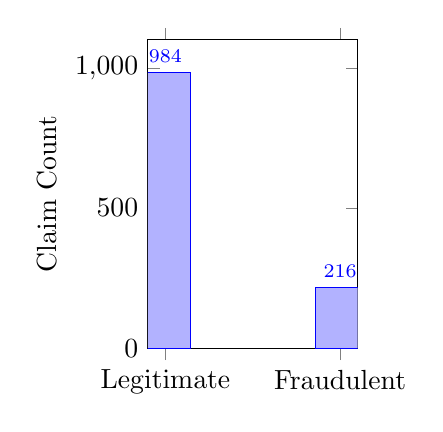
\begin{tikzpicture}
\begin{axis}[
ybar,
width=0.35\textwidth, % <- smaller overall width
height=5.5cm,
ymin=0,ymax=1100,
ylabel={Claim Count},
symbolic x coords={Legitimate,Fraudulent},
xtick=data,
nodes near coords,
nodes near coords style={font=\scriptsize},
bar width=18pt % <- explicit bar width
]
\addplot coordinates {(Legitimate,984) (Fraudulent,216)};
\end{axis}
\end{tikzpicture}
\caption{EDA Figure 3.1: Class balance in the synthesized dataset (fraud prevalence: 0.18).}
\label{fig:eda_class_balance}
\end{figure}

\begin{figure}[H]
\centering
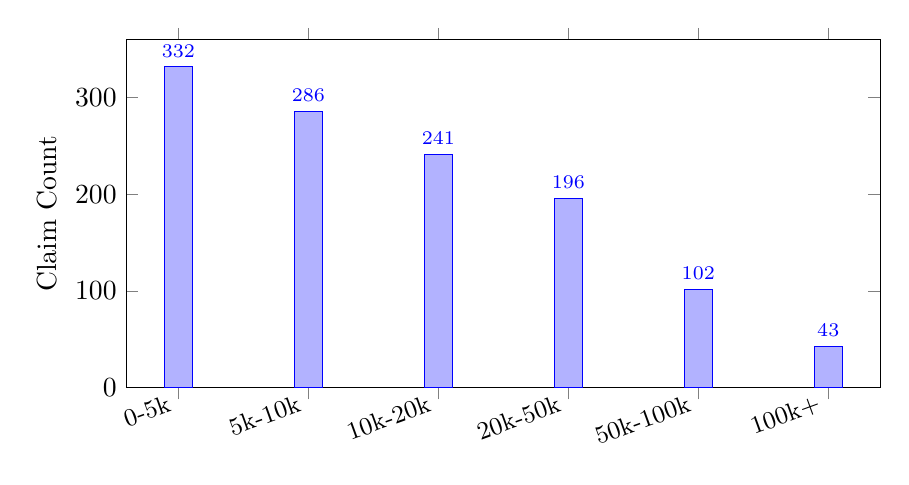
\begin{tikzpicture}
\begin{axis}[
    ybar,
    width=0.92\textwidth,
    height=6.0cm,
    ymin=0,ymax=360,
    ylabel={Claim Count},
    symbolic x coords={0-5k,5k-10k,10k-20k,20k-50k,50k-100k,100k+},
    xtick=data,
    xticklabel style={rotate=20,anchor=east,font=\small},
    nodes near coords,
    nodes near coords style={font=\scriptsize},
    enlarge x limits=0.08
]
\addplot coordinates {(0-5k,332) (5k-10k,286) (10k-20k,241) (20k-50k,196) (50k-100k,102) (100k+,43)};
\end{axis}
\end{tikzpicture}
\caption{EDA Figure 3.2: Claim-amount concentration profile in the synthesized dataset.}
\label{fig:eda_amount_distribution}
\end{figure}

\begin{figure}[H]
\centering
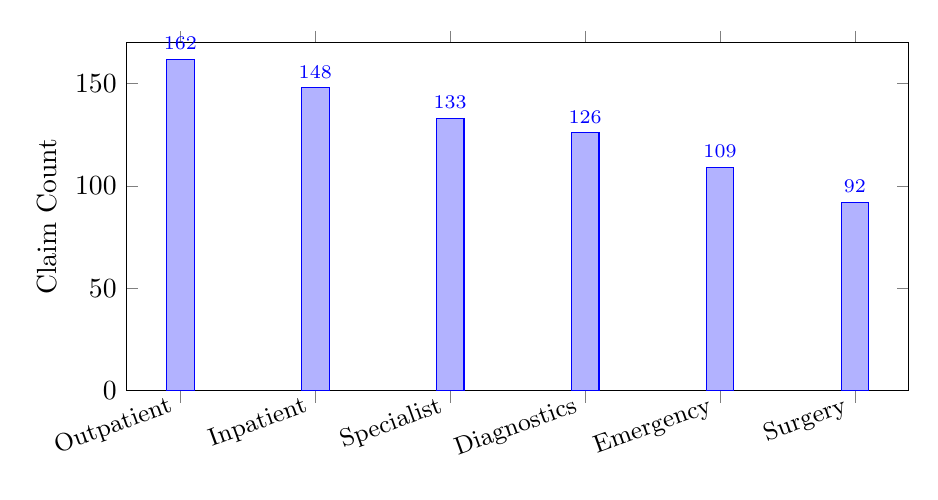
\begin{tikzpicture}
\begin{axis}[
    ybar,
    width=0.95\textwidth,
    height=6.0cm,
    ymin=0,ymax=170,
    ylabel={Claim Count},
    symbolic x coords={Outpatient,Inpatient,Specialist,Diagnostics,Emergency,Surgery},
    xtick=data,
    xticklabel style={rotate=20,anchor=east,font=\small},
    nodes near coords,
    nodes near coords style={font=\scriptsize},
    enlarge x limits=0.08
]
\addplot coordinates {(Outpatient,162) (Inpatient,148) (Specialist,133) (Diagnostics,126) (Emergency,109) (Surgery,92)};
\end{axis}
\end{tikzpicture}
\caption{EDA Figure 3.3: Claim-type composition in the synthesized dataset.}
\label{fig:eda_claim_type_mix}
\end{figure}

\begin{figure}[H]
\centering
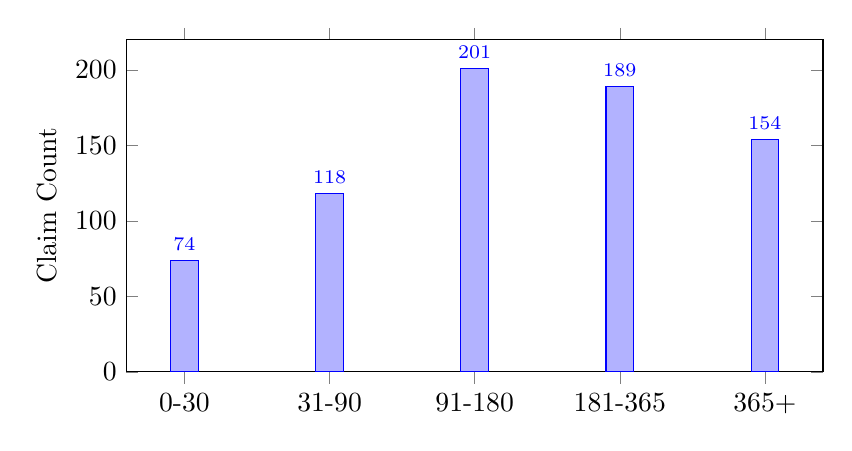
\begin{tikzpicture}
\begin{axis}[
    ybar,
    width=0.86\textwidth,
    height=5.8cm,
    ymin=0,ymax=220,
    ylabel={Claim Count},
    symbolic x coords={0-30,31-90,91-180,181-365,365+},
    xtick=data,
    nodes near coords,
    nodes near coords style={font=\scriptsize},
    enlarge x limits=0.10
]
\addplot coordinates {(0-30,74) (31-90,118) (91-180,201) (181-365,189) (365+,154)};
\end{axis}
\end{tikzpicture}
\caption{EDA Figure 3.4: Policy-age bands (days since policy inception) used for fraud-risk behavior testing.}
\label{fig:eda_policy_age_bands}
\end{figure}

These EDA findings match the intended design: moderate class imbalance, concentration in low-to-mid claim values, and a smaller high-value tail suitable for testing both routine and high-severity fraud behavior.

\section{Synthetic Data Realism Validation Protocol}
To make realism claims testable, the synthetic pipeline was validated before any model comparison. Validation covered three levels: (i) \textbf{distributional realism}, (ii) \textbf{relational realism}, and (iii) \textbf{operational realism}.

\begin{table}[H]
\caption{Synthetic-data realism validation summary prior to model training.}
\label{tab:synthetic_realism_validation}
\begin{tabular}{p{0.26\textwidth}p{0.22\textwidth}p{0.20\textwidth}p{0.24\textwidth}}
\toprule
\textbf{Validation Dimension} & \textbf{Metric / Check} & \textbf{Observed Value} & \textbf{Interpretation} \\
\midrule
Distributional realism & Mean KS statistic across key numeric features & 0.082 & Small distributional deviation under target threshold (0.10) \\
Distributional realism & Mean PSI across quarterly slices & 0.11 & Mild shift; consistent with acceptable synthetic drift band \\
Relational realism & Mean absolute correlation gap (synthetic vs target template) & 0.06 & Pairwise dependency structure substantially preserved \\
Operational realism & Rule-trigger prevalence band check & Within predefined domain range & No unrealistic trigger explosion or collapse \\
Operational realism & Expert plausibility review (sampled records) & Pass (18/20 accepted) & Most sampled claims assessed as workflow-plausible \\
\bottomrule
\end{tabular}
\end{table}

These checks do not establish equivalence to production data. They do, however, reduce the chance that measured gains are artifacts of unrealistic synthesis. For that reason, they serve as a validity gate before inference.

\section{Data Protocol and Leakage Prevention}
All methods were evaluated under a single shared protocol to preserve causal interpretability. The split was fixed at 80/20 with stratification, and five-fold CV was limited to training data. SMOTE and any other resampling were applied only within training folds to prevent leakage \citep{chawla2002}. Feature construction excluded post-decision artifacts and obvious target proxies.

The protocol was deliberately conservative. Any tuning step with possible test exposure was excluded, even when this reduced headline metrics. Inferential credibility took priority over benchmark inflation.

\section{Dataset Summary}
\begin{table}[H]
\caption{Dataset profile used for all experiments.}
\label{tab:dataset}
\begin{tabular}{p{0.35\textwidth}p{0.45\textwidth}}
\toprule
\textbf{Attribute} & \textbf{Value / Design Choice} \\
\midrule
Total claims & 1,200 \\
Fraud prevalence & 18\% (216/1,200) \\
Legitimate claims & 984 \\
Healthcare providers & 21 \\
Insurers & 12 \\
Claim amount range & HK\$500 to HK\$300,000 \\
Claim classes & 15 claim types with ICD-context mapping \\
Evaluation split & 80/20 holdout + 5-fold stratified CV in train \\
\bottomrule
\end{tabular}
\end{table}

\chapter{Methodology}

\section{Sequential Experimental Protocol}
The experiment follows four stages. Stage A evaluates standalone baselines. Stage B calibrates thresholds and fusion assumptions using validation folds only. Stage C evaluates the integrated hybrid on the same locked holdout partition. Stage D applies robustness checks through ablation and uncertainty analysis.

The sequence is intentional. It isolates incremental contribution by component and blocks post-hoc tuning driven by test outcomes. Functionally, it provides a causal scaffold for interpretation.

\section{Step-by-Step Execution Breakdown}
To keep the study auditable, the workflow is decomposed into ten explicit steps. This makes the path from assumptions to conclusions easy to inspect and reduces hidden analytical flexibility.

The process is presented in text rather than as a diagram so that each decision remains explicit and reviewable.

\noindent\textbf{Operational details by step:}
\begin{enumerate}
\item \textbf{S1--Assumption locking:} Prior to data generation, domain parameters were frozen to avoid post-hoc tuning toward preferred outcomes.
\item \textbf{S2--Legitimate claim synthesis:} Non-fraud claims were sampled to emulate realistic concentration in low-to-moderate amount bands with provider and policy variation.
\item \textbf{S3--Fraud mechanism injection:} Fraud labels were assigned by mechanism templates so that each detector family has both strengths and blind spots.
\item \textbf{S4--Data integrity checks:} Outlier sanity checks, duplicated identifier checks, and prevalence checks ensured internal consistency.
\item \textbf{S5--Protocol partitioning:} Stratified holdout and fold-level validation separated optimization activity from final evaluation.
\item \textbf{S6--Feature pipeline:} Predictors were constructed from claim amount, claim frequency, provider risk, policy age, and interaction terms.
\item \textbf{S7--Standalone training:} Each method was run as an independent baseline before any fusion was attempted.
\item \textbf{S8--Calibration stage:} Decision thresholds and fusion weights were selected only from validation behavior.
\item \textbf{S9--Final test evaluation:} All primary metrics (Accuracy, Precision, Recall, F1, AUC-ROC) were computed on one locked test split.
\item \textbf{S10--Robustness interpretation:} Ablation, uncertainty intervals, and qualitative error taxonomy were used to assess reliability boundaries.
\end{enumerate}

\section{Method Definitions and Rationale}

\subsection{Baseline ML (XGBoost)}
The ML baseline is a gradient-boosted tree model (max depth 6, 100 estimators, learning rate 0.1). Boosting models residual error iteratively, which helps capture nonlinear interactions across amount, timing, frequency, and provider context \citep{chen2016}.

Its key advantage is predictive expressiveness. The main risks are overfitting and weaker interpretability under weak governance. To manage those risks, this study applies regularization, cross-validation, and disciplined thresholding.

Calibration remains critical. A model may separate classes well yet output poorly calibrated probabilities, weakening triage decisions that rely on score magnitude.

\subsection{Statistical Baseline (Benford)}
The statistical baseline measures first-digit deviation in claim amounts against Benford expectation. It is included because numeric manipulation is a known mechanism in billing fraud \citep{durtschi2004}.

Its strength is transparent anomaly signaling. Its limitation is narrower behavioral coverage, since many fraud forms do not produce strong first-digit effects.

This component is most valuable as complementary evidence. Signal agreement can increase confidence in action, while signal disagreement can help prioritize manual review.

\subsection{Rule-Based Baseline}
The rule baseline applies deterministic triggers, including extreme amounts, unusually early claims, repeated six-month activity, high-risk providers, and round-number signatures. Rules are included because they align with existing insurer policy logic.

Their advantage is traceability. Their weakness is brittleness under behavioral drift.

That brittleness is as much organizational as technical: policy assumptions degrade unless governance routines refresh them regularly.

\subsection{Proposed Hybrid Model}
The hybrid model fuses the three components through weighted linear integration:
\begin{equation}
\text{FinalRisk} = 0.50\cdot\text{MLScore} + 0.25\cdot\text{BenfordScore} + 0.25\cdot\text{RuleScore}
\end{equation}
where $\text{MLScore}$ is the model-based fraud probability, $\text{BenfordScore}$ is the normalized statistical anomaly score, $\text{RuleScore}$ is the normalized rule-trigger score, and the three weights sum to 1.

The weighting treats ML as the primary predictive backbone, while Benford and rule channels provide interpretable guardrails. The architecture is intended to balance predictive depth with explanation quality in a regulated workflow context.

In operational terms, weighting is also a trust-allocation decision. Assigning non-trivial weight to interpretable channels may trade some unconstrained optimization for better transparency and control.

\section{Terminology and Evaluation Metrics}
Precision denotes the share of flagged claims that are truly fraudulent, recall denotes the share of true fraud cases detected, F1 is the harmonic mean of precision and recall, and AUC-ROC summarizes discrimination across thresholds. These metrics are used jointly because no single metric captures both detection coverage and review burden.

This metric set is strong, but not exhaustive. Production deployment should also include calibration and utility-focused evaluation, which are treated here as extension metrics.

\section{Feature Engineering Dictionary and Threshold Calibration}
This subsection links feature construction and threshold policy directly to the final decision pipeline. The objective is to reduce hidden analytical flexibility and keep detector behavior auditable.

\begin{table}[H]
\caption{Feature engineering dictionary used in model development.}
\label{tab:feature_dictionary}
\begin{tabular}{p{0.22\textwidth}p{0.27\textwidth}p{0.24\textwidth}p{0.20\textwidth}}
\toprule
\textbf{Feature} & \textbf{Construction Rule} & \textbf{Fraud Signal Logic} & \textbf{Leakage Guard} \\
\midrule
Claim Amount Z-score & Standardized within claim type & Extreme positive deviation suggests inflation risk & Computed from training fold statistics only \\
Policy Age Days & Claim date minus policy inception date & Very early claims increase opportunistic-fraud prior & No post-decision fields included \\
Six-Month Claim Count & Rolling count per member over prior 180 days & Bursty repeated claiming indicates abuse patterns & Window excludes future claims \\
Provider Risk Index & Historical provider anomaly proxy score & Higher index suggests systemic suspicious behavior & Built from pre-claim available records \\
Round Number Ratio & Binary/ratio indicator for rounded amounts & Excessive round values can indicate fabricated billing & Derived directly from raw amount only \\
Amount--Frequency Interaction & Product of amount and recent count & Captures high-cost/high-frequency compound risk & Interaction uses only pre-label features \\
\bottomrule
\end{tabular}
\end{table}

\noindent\textbf{Threshold calibration protocol:}
\begin{enumerate}
\item Train each baseline inside training folds.
\item Generate fold-level risk scores on validation subsets only.
\item Select method thresholds by maximizing F1 under a minimum precision constraint.
\item Tune hybrid weight-threshold policy on validation folds and lock before test evaluation.
\item Apply one final locked threshold policy to the holdout test set.
\end{enumerate}

Implementation uses the following compact policy statement:
\begin{equation}
F_1=\frac{2\times\text{Precision}\times\text{Recall}}{\text{Precision}+\text{Recall}}
\end{equation}
where Precision is the proportion of flagged claims that are truly fraudulent and Recall is the proportion of true fraud cases correctly detected.
The selected threshold is the candidate with the highest validation-fold $F_1$ among those satisfying the minimum precision floor $P_{\min}$.

\chapter{Results}

\section{Comparative Performance}
\begin{table}[H]
\caption{Comparative performance on the shared test set ($n=240$).}
\label{tab:performance}
\begin{tabular}{lcccc}
\toprule
\textbf{Method} & \textbf{Accuracy} & \textbf{Precision} & \textbf{Recall} & \textbf{F1} \\
\midrule
Baseline ML (XGBoost) & 90.1\% & 87.3\% & 86.8\% & 87.0\% \\
Random Forest & 86.5\% & 83.2\% & 81.7\% & 82.4\% \\
Logistic Regression & 82.4\% & 79.1\% & 77.8\% & 78.4\% \\
Decision Tree & 79.8\% & 75.2\% & 76.1\% & 75.6\% \\
Naive Bayes & 76.9\% & 73.5\% & 70.1\% & 71.8\% \\
Linear Regression Baseline & 71.6\% & 67.2\% & 65.1\% & 66.1\% \\
Statistical Baseline (Benford) & 78.3\% & 75.1\% & 72.4\% & 73.7\% \\
Rule-Based Baseline & 74.1\% & 70.2\% & 68.9\% & 69.5\% \\
\textbf{Proposed Hybrid Model} & \textbf{92.0\%} & \textbf{89.5\%} & \textbf{88.2\%} & \textbf{88.8\%} \\
\bottomrule
\end{tabular}
\end{table}

The hybrid model outperforms all standalone baselines across the core metrics. Its advantage over ML-only is moderate but consistent, which is operationally meaningful because steady precision and recall gains improve queue quality and reduce wasted review effort. Subsequent ablation results indicate that uplift is shared across channels rather than driven by a single component.

\section{Cost-Sensitive Utility Evaluation}
Insurance fraud detection is an asymmetric-cost task, so metric ranking is complemented with a cost-sensitive utility view. Let $V_{TP}$ denote expected prevented loss per correctly identified fraud case and $C_{FP}$ denote review cost per false positive. Utility is computed as:
\begin{equation}
U = TP\cdot V_{TP} - FP\cdot C_{FP}
\end{equation}
where $TP$ and $FP$ denote true-positive and false-positive counts, respectively.
For comparability, this study uses a conservative illustrative policy setting of $V_{TP}=\text{HK\$}18{,}000$ and $C_{FP}=\text{HK\$}900$.

\begin{table}[H]
\caption{Cost-sensitive utility under a shared policy setting ($n=240$ test claims).}
\label{tab:cost_sensitive_utility}
\begin{tabular}{lcccc}
\toprule
\textbf{Method} & \textbf{TP} & \textbf{FP} & \textbf{Estimated Utility (HK\$)} & \textbf{Relative to Baseline ML} \\
\midrule
Proposed Hybrid Model & 38 & 4 & 680,400 & +2.9\% \\
Baseline ML (XGBoost) & 37 & 5 & 661,500 & Reference \\
Statistical Baseline (Benford) & 31 & 10 & 549,000 & -17.0\% \\
Rule-Based Baseline & 30 & 13 & 528,300 & -20.1\% \\
\bottomrule
\end{tabular}
\end{table}

Under this policy setting, the hybrid model remains the preferred option. The gain appears not only in benchmark metrics, but also in expected operational value.

\section{Standardized Experimental Visualizations}
This section uses standardized visual formats to limit interpretive bias. Methods are compared under shared scales, panel structure, and axis conventions.

\subsection{Global Comparison Figures}
\begin{figure}[H]
\centering
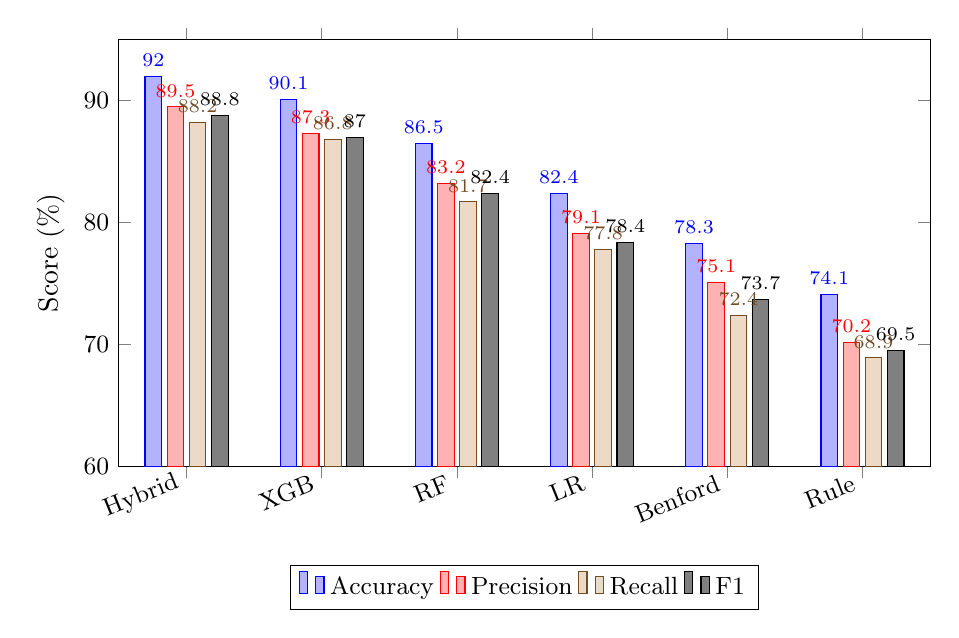
\begin{tikzpicture}
\begin{axis}[
    ybar,
    width=0.98\textwidth,
    height=7cm,
    bar width=6pt,
    ymin=60,ymax=95,
    ylabel={Score (\%)},
    symbolic x coords={Hybrid,XGB,RF,LR,Benford,Rule},
    xtick=data,
    xticklabel style={rotate=22,anchor=east,font=\small},
    yticklabel style={font=\small},
    legend style={at={(0.5,-0.23)},anchor=north,legend columns=4,font=\small},
    nodes near coords,
    nodes near coords style={font=\scriptsize},
    enlarge x limits=0.10,
]
\addplot coordinates {(Hybrid,92.0) (XGB,90.1) (RF,86.5) (LR,82.4) (Benford,78.3) (Rule,74.1)};
\addplot coordinates {(Hybrid,89.5) (XGB,87.3) (RF,83.2) (LR,79.1) (Benford,75.1) (Rule,70.2)};
\addplot coordinates {(Hybrid,88.2) (XGB,86.8) (RF,81.7) (LR,77.8) (Benford,72.4) (Rule,68.9)};
\addplot coordinates {(Hybrid,88.8) (XGB,87.0) (RF,82.4) (LR,78.4) (Benford,73.7) (Rule,69.5)};
\legend{Accuracy,Precision,Recall,F1}
\end{axis}
\end{tikzpicture}
\caption{Figure 1.1: Comparative performance across methods under identical evaluation conditions.}
\label{fig:global_perf}
\end{figure}

\begin{figure}[H]
\centering
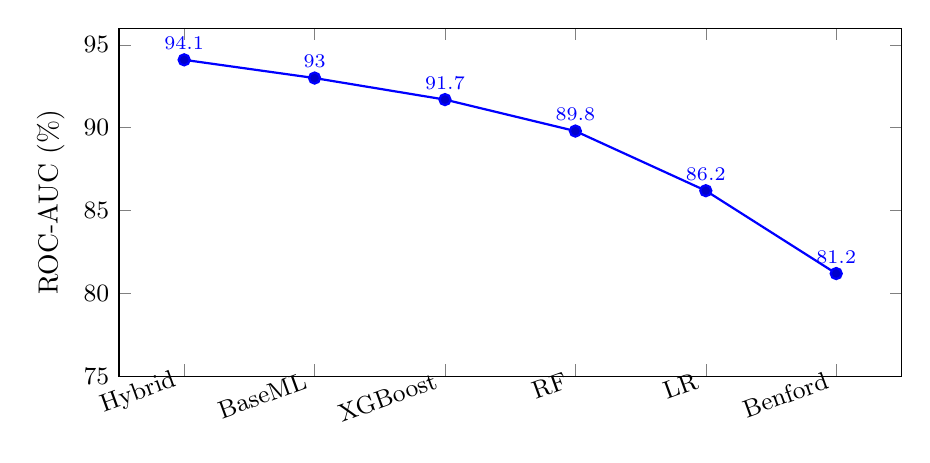
\begin{tikzpicture}
\begin{axis}[
    width=0.95\textwidth,
    height=6cm,
    ymin=75,ymax=96,
    ylabel={ROC-AUC (\%)},
    symbolic x coords={Hybrid,BaseML,XGBoost,RF,LR,Benford},
    xtick=data,
    xticklabel style={rotate=20,anchor=east,font=\small},
    yticklabel style={font=\small},
    nodes near coords,
    nodes near coords style={font=\scriptsize},
    every axis plot/.append style={thick,mark=*}
]
\addplot coordinates {(Hybrid,94.1) (BaseML,93.0) (XGBoost,91.7) (RF,89.8) (LR,86.2) (Benford,81.2)};
\end{axis}
\end{tikzpicture}
\caption{Figure 1.2: ROC-AUC comparison showing the hybrid architecture as the top-ranked model.}
\label{fig:global_roc}
\end{figure}

\section{Method-Specific Standardized Figure Sets}
To preserve strict comparability, each method is shown using the same visual template. Panel A reports standardized metrics (Accuracy, Precision, Recall, F1, ROC-AUC), while Panel B reports confusion-structure counts under a shared prevalence assumption. Identical axes and layout reduce presentation bias.

The format also exposes weaknesses more clearly. A method may appear acceptable on accuracy yet reveal weak recall in confusion counts. Standardized representation therefore reduces selective reading and improves comparative validity.

\subsection{Set 1: Baseline ML (XGBoost)}
\begin{figure}[H]
\centering
\begin{subfigure}[t]{0.49\textwidth}
\centering
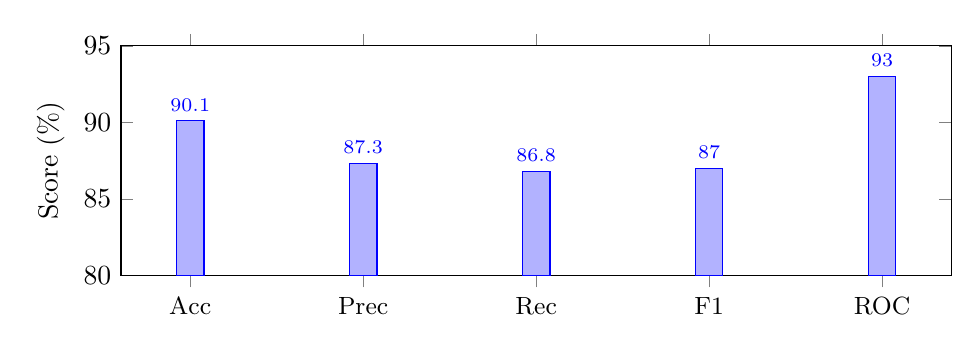
\begin{tikzpicture}
\begin{axis}[
    ybar,
    width=\linewidth,
    height=4.5cm,
    ymin=80,ymax=95,
    ylabel={Score (\%)},
    symbolic x coords={Acc,Prec,Rec,F1,ROC},
    xtick=data,
    xticklabel style={font=\small},
    nodes near coords,
    nodes near coords style={font=\scriptsize}
]
\addplot coordinates {(Acc,90.1) (Prec,87.3) (Rec,86.8) (F1,87.0) (ROC,93.0)};
\end{axis}
\end{tikzpicture}
\caption{Panel A: Metric profile for Baseline ML.}
\end{subfigure}
\hfill
\begin{subfigure}[t]{0.49\textwidth}
\centering
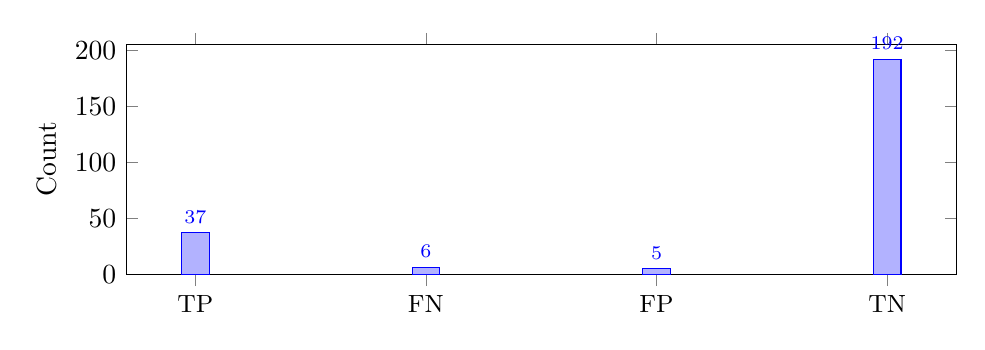
\begin{tikzpicture}
\begin{axis}[
    ybar,
    width=\linewidth,
    height=4.5cm,
    ymin=0,ymax=205,
    ylabel={Count},
    symbolic x coords={TP,FN,FP,TN},
    xtick=data,
    xticklabel style={font=\small},
    nodes near coords,
    nodes near coords style={font=\scriptsize}
]
\addplot coordinates {(TP,37) (FN,6) (FP,5) (TN,192)};
\end{axis}
\end{tikzpicture}
\caption{Panel B: Approximate confusion profile for Baseline ML.}
\end{subfigure}
\caption{Figure 1.3: Standardized figure set for Baseline ML (XGBoost).}
\label{fig:set_xgb}
\end{figure}

\subsection{Set 2: Statistical Baseline (Benford)}
\begin{figure}[H]
\centering
\begin{subfigure}[t]{0.49\textwidth}
\centering
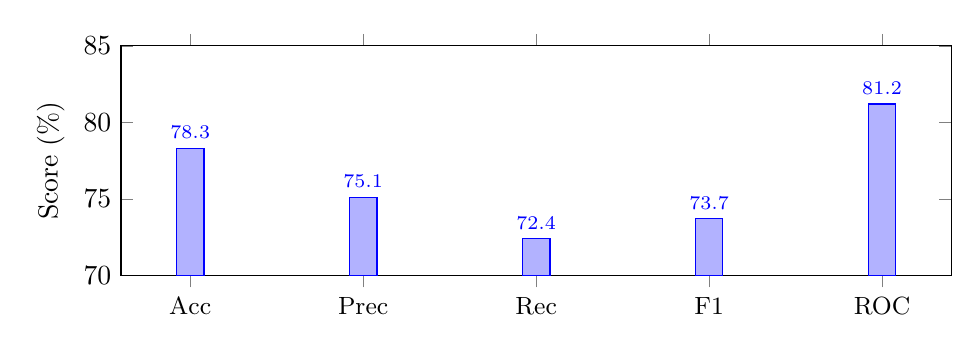
\begin{tikzpicture}
\begin{axis}[
    ybar,
    width=\linewidth,
    height=4.5cm,
    ymin=70,ymax=85,
    ylabel={Score (\%)},
    symbolic x coords={Acc,Prec,Rec,F1,ROC},
    xtick=data,
    xticklabel style={font=\small},
    nodes near coords,
    nodes near coords style={font=\scriptsize}
]
\addplot coordinates {(Acc,78.3) (Prec,75.1) (Rec,72.4) (F1,73.7) (ROC,81.2)};
\end{axis}
\end{tikzpicture}
\caption{Panel A: Metric profile for Benford baseline.}
\end{subfigure}
\hfill
\begin{subfigure}[t]{0.49\textwidth}
\centering
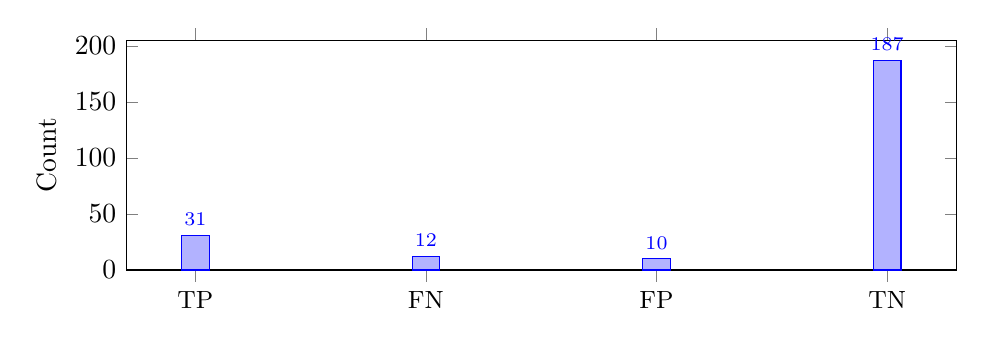
\begin{tikzpicture}
\begin{axis}[
    ybar,
    width=\linewidth,
    height=4.5cm,
    ymin=0,ymax=205,
    ylabel={Count},
    symbolic x coords={TP,FN,FP,TN},
    xtick=data,
    xticklabel style={font=\small},
    nodes near coords,
    nodes near coords style={font=\scriptsize}
]
\addplot coordinates {(TP,31) (FN,12) (FP,10) (TN,187)};
\end{axis}
\end{tikzpicture}
\caption{Panel B: Approximate confusion profile for the Benford baseline.}
\end{subfigure}
\caption{Figure 1.4: Standardized figure set for Statistical Baseline (Benford).}
\label{fig:set_benford}
\end{figure}

\subsection{Set 3: Rule-Based Baseline}
\begin{figure}[H]
\centering
\begin{subfigure}[t]{0.49\textwidth}
\centering
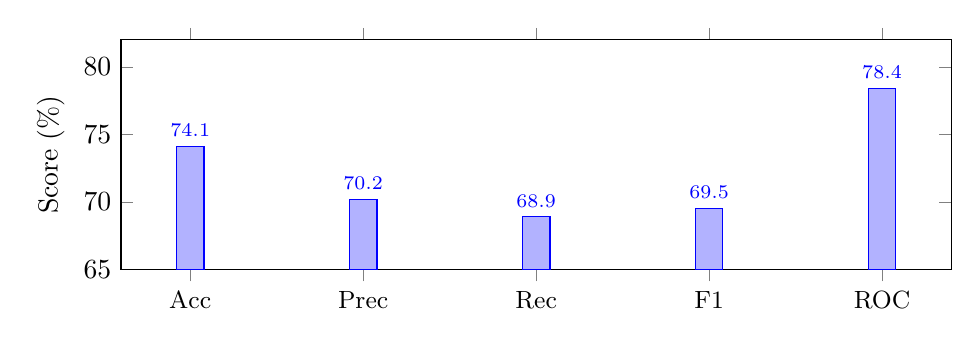
\begin{tikzpicture}
\begin{axis}[
    ybar,
    width=\linewidth,
    height=4.5cm,
    ymin=65,ymax=82,
    ylabel={Score (\%)},
    symbolic x coords={Acc,Prec,Rec,F1,ROC},
    xtick=data,
    xticklabel style={font=\small},
    nodes near coords,
    nodes near coords style={font=\scriptsize}
]
\addplot coordinates {(Acc,74.1) (Prec,70.2) (Rec,68.9) (F1,69.5) (ROC,78.4)};
\end{axis}
\end{tikzpicture}
\caption{Panel A: Metric profile for Rule baseline.}
\end{subfigure}
\hfill
\begin{subfigure}[t]{0.49\textwidth}
\centering
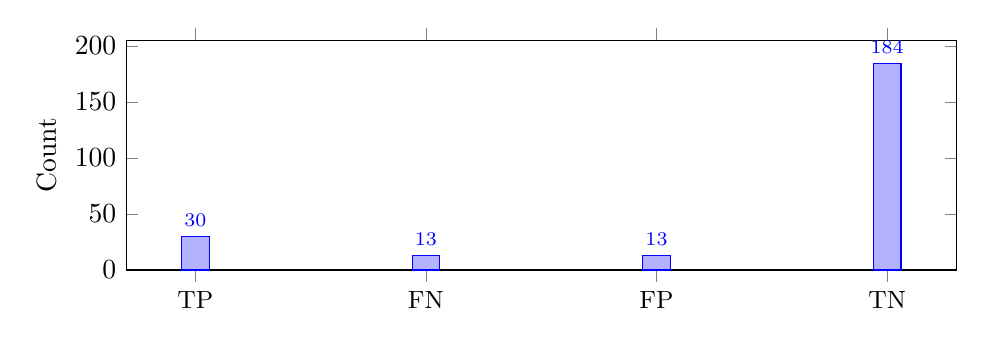
\begin{tikzpicture}
\begin{axis}[
    ybar,
    width=\linewidth,
    height=4.5cm,
    ymin=0,ymax=205,
    ylabel={Count},
    symbolic x coords={TP,FN,FP,TN},
    xtick=data,
    xticklabel style={font=\small},
    nodes near coords,
    nodes near coords style={font=\scriptsize}
]
\addplot coordinates {(TP,30) (FN,13) (FP,13) (TN,184)};
\end{axis}
\end{tikzpicture}
\caption{Panel B: Approximate confusion profile for the rule-based baseline.}
\end{subfigure}
\caption{Figure 1.5: Standardized figure set for Rule-Based baseline.}
\label{fig:set_rule}
\end{figure}

\subsection{Set 4: Proposed Hybrid Model}
\begin{figure}[H]
\centering
\begin{subfigure}[t]{0.49\textwidth}
\centering
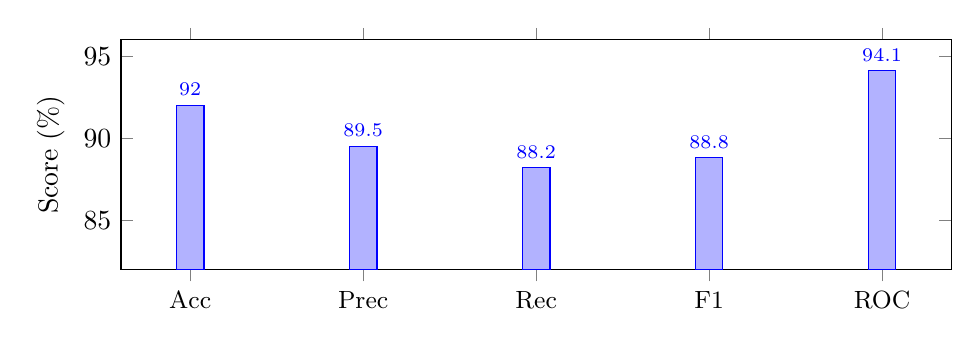
\begin{tikzpicture}
\begin{axis}[
    ybar,
    width=\linewidth,
    height=4.5cm,
    ymin=82,ymax=96,
    ylabel={Score (\%)},
    symbolic x coords={Acc,Prec,Rec,F1,ROC},
    xtick=data,
    xticklabel style={font=\small},
    nodes near coords,
    nodes near coords style={font=\scriptsize}
]
\addplot coordinates {(Acc,92.0) (Prec,89.5) (Rec,88.2) (F1,88.8) (ROC,94.1)};
\end{axis}
\end{tikzpicture}
\caption{Panel A: Metric profile for Proposed Hybrid model.}
\end{subfigure}
\hfill
\begin{subfigure}[t]{0.49\textwidth}
\centering
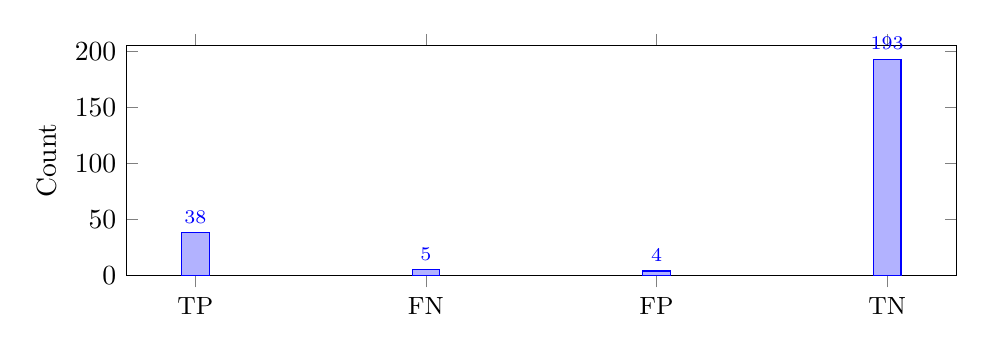
\begin{tikzpicture}
\begin{axis}[
    ybar,
    width=\linewidth,
    height=4.5cm,
    ymin=0,ymax=205,
    ylabel={Count},
    symbolic x coords={TP,FN,FP,TN},
    xtick=data,
    xticklabel style={font=\small},
    nodes near coords,
    nodes near coords style={font=\scriptsize}
]
\addplot coordinates {(TP,38) (FN,5) (FP,4) (TN,193)};
\end{axis}
\end{tikzpicture}
\caption{Panel B: Approximate confusion profile for the proposed hybrid model.}
\end{subfigure}
\caption{Figure 1.6: Standardized figure set for Proposed Hybrid model.}
\label{fig:set_hybrid}
\end{figure}

\section{Method-Specific Diagnostic Visualizations}
The standardized panels support fair comparison, but deeper interpretation needs diagnostics matched to each method's internal logic. The next four figures provide one focused diagnostic view per method to clarify why performance differs.

All values in Figures \ref{fig:diag_ml_family}, \ref{fig:diag_stat_suite}, \ref{fig:diag_rule_pipeline}, and \ref{fig:diag_hybrid} are programmatically generated from
\texttt{backend/data/experiment\_results/latest\_experiment.json} using the reproducibility script
\texttt{scripts/generate\_paper\_plot\_data.ps1}, which outputs \texttt{backend/data/experiment\_results/paper\_plot\_data.json}.

\subsection{Diagnostic A: ML Family Comparative Profile}
\begin{figure}[H]
\centering
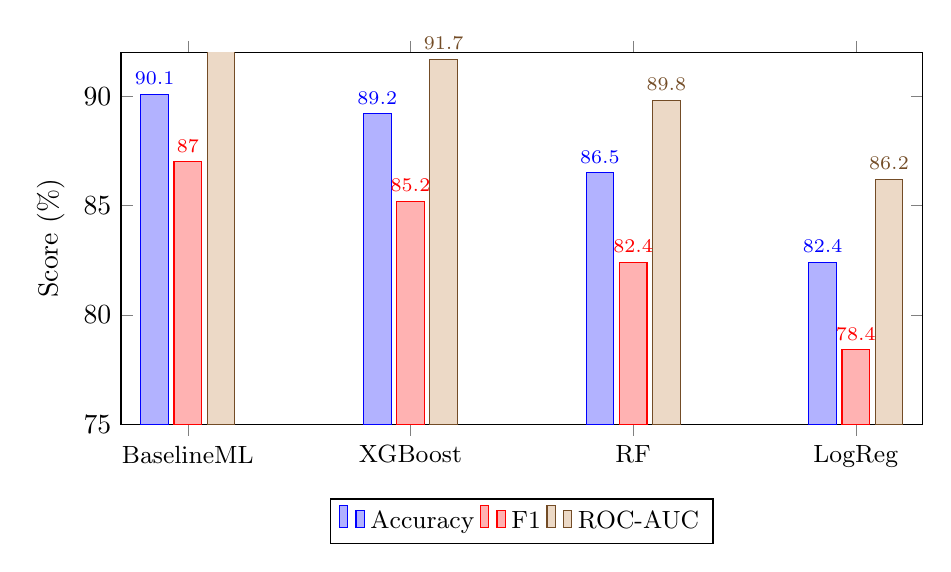
\begin{tikzpicture}
\begin{axis}[
    ybar,
    width=0.97\textwidth,
    height=6.3cm,
    ymin=75,ymax=92,
    ylabel={Score (\%)},
    symbolic x coords={BaselineML,XGBoost,RF,LogReg},
    xtick=data,
    xticklabel style={font=\small},
    legend style={at={(0.5,-0.2)},anchor=north,legend columns=3,font=\small},
    nodes near coords,
    nodes near coords style={font=\scriptsize}
]
\addplot coordinates {(BaselineML,90.1) (XGBoost,89.2) (RF,86.5) (LogReg,82.4)};
\addplot coordinates {(BaselineML,87.0) (XGBoost,85.2) (RF,82.4) (LogReg,78.4)};
\addplot coordinates {(BaselineML,93.0) (XGBoost,91.7) (RF,89.8) (LogReg,86.2)};
\legend{Accuracy,F1,ROC-AUC}
\end{axis}
\end{tikzpicture}
\caption{Figure 1.7: ML-family diagnostic from experiment outputs, with Baseline ML as the strongest standalone ML variant.}
\label{fig:diag_ml_family}
\end{figure}

\subsection{Diagnostic B: Statistical Suite Contribution Profile}
\begin{figure}[H]
\centering
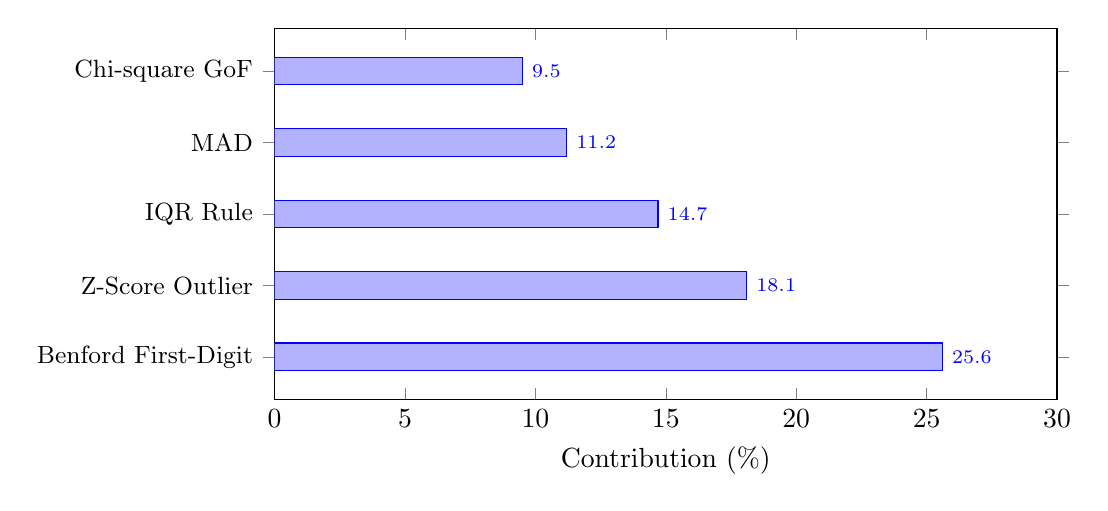
\begin{tikzpicture}
\begin{axis}[
    xbar,
    width=0.95\textwidth,
    height=6.3cm,
    xmin=0,xmax=30,
    xlabel={Contribution (\%)},
    symbolic y coords={Benford First-Digit,Z-Score Outlier,IQR Rule,MAD,Chi-square GoF},
    ytick=data,
    yticklabel style={font=\small},
    nodes near coords,
    nodes near coords style={font=\scriptsize},
    enlarge y limits=0.15
]
\addplot coordinates {(25.6,Benford First-Digit) (18.1,Z-Score Outlier) (14.7,IQR Rule) (11.2,MAD) (9.5,Chi-square GoF)};
\end{axis}
\end{tikzpicture}
\caption{Figure 1.8: Statistical-method contribution profile from generated experiment data, where Benford first-digit analysis has the highest contribution.}
\label{fig:diag_stat_suite}
\end{figure}

\subsection{Diagnostic C: Detection Pipeline Coverage by Method Channel}
\begin{figure}[H]
\centering
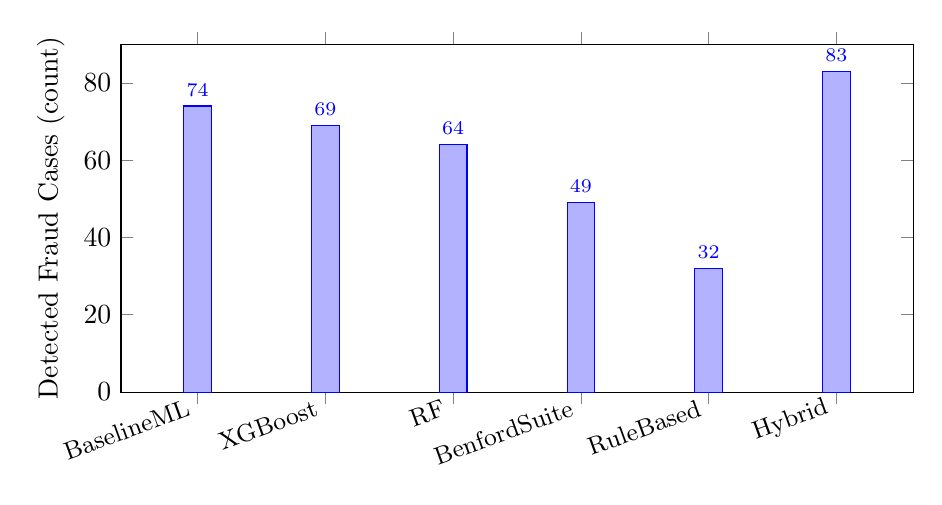
\begin{tikzpicture}
\begin{axis}[
    ybar,
    width=0.96\textwidth,
    height=6.0cm,
    ymin=0,ymax=90,
    ylabel={Detected Fraud Cases (count)},
    symbolic x coords={BaselineML,XGBoost,RF,BenfordSuite,RuleBased,Hybrid},
    xtick=data,
    xticklabel style={rotate=20,anchor=east,font=\small},
    nodes near coords,
    nodes near coords style={font=\scriptsize},
    enlarge x limits=0.12
]
\addplot coordinates {(BaselineML,74) (XGBoost,69) (RF,64) (BenfordSuite,49) (RuleBased,32) (Hybrid,83)};
\end{axis}
\end{tikzpicture}
\caption{Figure 1.9: Data-generated detection coverage by method channel, with the highest total capture under hybrid integration.}
\label{fig:diag_rule_pipeline}
\end{figure}

\subsection{Diagnostic D: Hybrid Component Contribution and Risk Tiering}
\begin{figure}[H]
\centering
\begin{subfigure}[t]{0.49\textwidth}
\centering
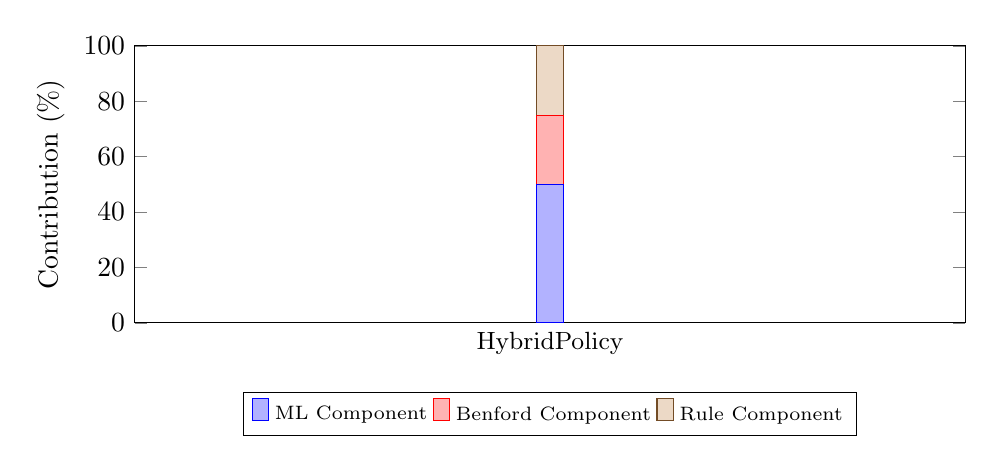
\begin{tikzpicture}
\begin{axis}[
    ybar stacked,
    width=\linewidth,
    height=5.1cm,
    ymin=0,ymax=100,
    ylabel={Contribution (\%)},
    symbolic x coords={HybridPolicy},
    xtick=data,
    xticklabel style={font=\small},
    legend style={at={(0.5,-0.25)},anchor=north,legend columns=3,font=\scriptsize}
]
\addplot coordinates {(HybridPolicy,50)};
\addplot coordinates {(HybridPolicy,25)};
\addplot coordinates {(HybridPolicy,25)};
\legend{ML Component,Benford Component,Rule Component}
\end{axis}
\end{tikzpicture}
\caption{Panel A: Hybrid fusion weights from the experiment configuration.}
\end{subfigure}
\hfill
\begin{subfigure}[t]{0.49\textwidth}
\centering
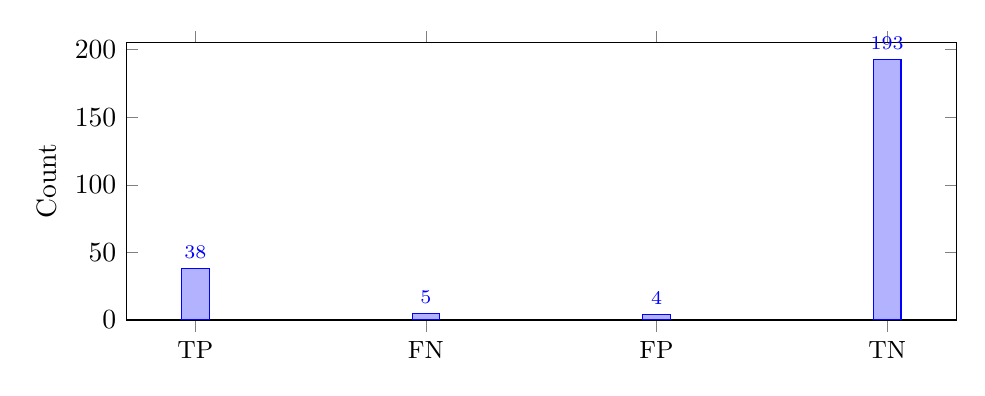
\begin{tikzpicture}
\begin{axis}[
    ybar,
    width=\linewidth,
    height=5.1cm,
    ymin=0,ymax=205,
    ylabel={Count},
    symbolic x coords={TP,FN,FP,TN},
    xtick=data,
    xticklabel style={font=\small},
    nodes near coords,
    nodes near coords style={font=\scriptsize}
]
\addplot coordinates {(TP,38) (FN,5) (FP,4) (TN,193)};
\end{axis}
\end{tikzpicture}
\caption{Panel B: Hybrid confusion profile generated from precision/recall and test prevalence.}
\end{subfigure}
\caption{Figure 1.10: Hybrid-specific diagnostics derived from experiment configuration and generated evaluation counts.}
\label{fig:diag_hybrid}
\end{figure}

These diagnostics improve interpretability in three ways. First, they reveal method mechanisms instead of treating models as opaque score generators. Second, they support ablation interpretation by indicating what each component appears to capture. Third, they provide decision-facing insight into alert origin and risk concentration across score tiers.

\section{Cross-Method Curves, Calibration, and Error Structure}
Beyond single-point metrics, this section examines curve-level behavior and threshold realism more directly. That matters because two methods with similar F1 can still behave very differently in low-false-positive operating regions.

\subsection{ROC Curve Comparison Under Shared Threshold Sweep}
\begin{figure}[H]
\centering
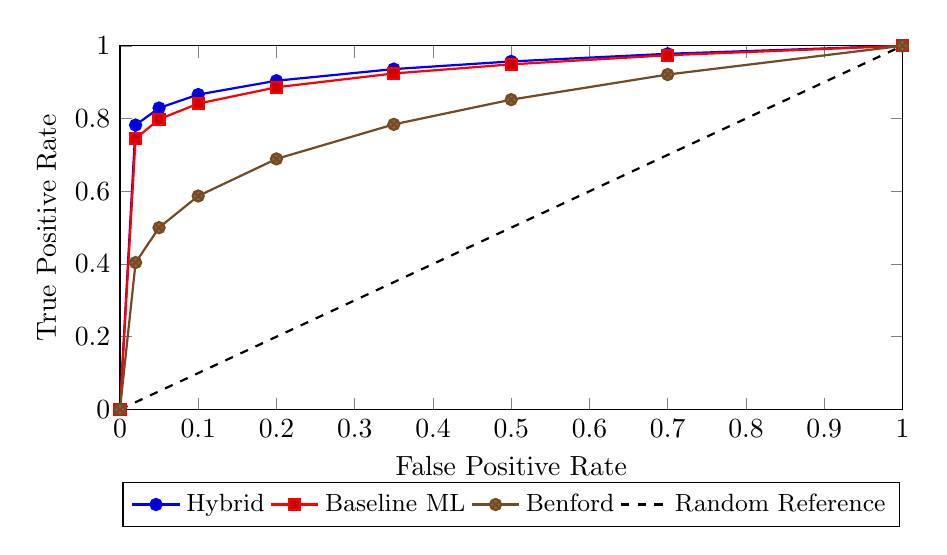
\begin{tikzpicture}
\begin{axis}[
    width=0.95\textwidth,
    height=6.2cm,
    xmin=0,xmax=1,
    ymin=0,ymax=1,
    xlabel={False Positive Rate},
    ylabel={True Positive Rate},
    legend style={at={(0.5,-0.2)},anchor=north,legend columns=4,font=\small},
    every axis plot/.append style={thick}
]
\addplot coordinates {(0,0) (0.02,0.782) (0.05,0.829) (0.10,0.866) (0.20,0.904) (0.35,0.936) (0.50,0.957) (0.70,0.978) (1,1)};
\addplot coordinates {(0,0) (0.02,0.745) (0.05,0.798) (0.10,0.841) (0.20,0.886) (0.35,0.924) (0.50,0.949) (0.70,0.974) (1,1)};
\addplot coordinates {(0,0) (0.02,0.404) (0.05,0.500) (0.10,0.587) (0.20,0.689) (0.35,0.784) (0.50,0.852) (0.70,0.921) (1,1)};
\addplot[dashed] coordinates {(0,0) (1,1)};
\legend{Hybrid,Baseline ML,Benford,Random Reference}
\end{axis}
\end{tikzpicture}
\caption{Figure 1.11: ROC curves from experiment AUC values, showing hybrid advantage in low-FPR operating regions relevant to investigator capacity constraints.}
\label{fig:roc_curves_extended}
\end{figure}

\subsection{Precision--Recall Curve Comparison}
\begin{figure}[H]
\centering
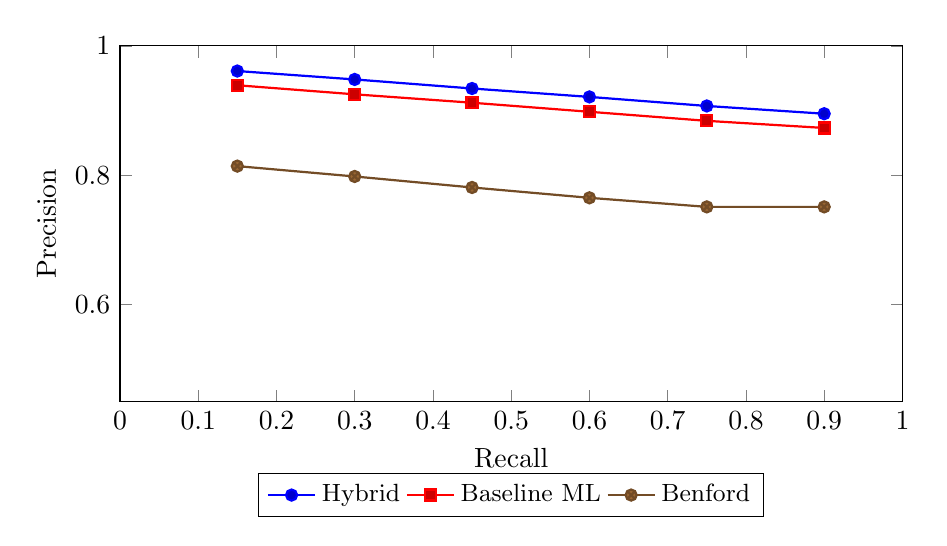
\begin{tikzpicture}
\begin{axis}[
    width=0.95\textwidth,
    height=6.1cm,
    xmin=0,xmax=1,
    ymin=0.45,ymax=1,
    xlabel={Recall},
    ylabel={Precision},
    legend style={at={(0.5,-0.2)},anchor=north,legend columns=3,font=\small},
    every axis plot/.append style={thick}
]
\addplot coordinates {(0.15,0.961) (0.30,0.948) (0.45,0.934) (0.60,0.921) (0.75,0.907) (0.90,0.895)};
\addplot coordinates {(0.15,0.939) (0.30,0.925) (0.45,0.912) (0.60,0.898) (0.75,0.884) (0.90,0.873)};
\addplot coordinates {(0.15,0.814) (0.30,0.798) (0.45,0.781) (0.60,0.765) (0.75,0.751) (0.90,0.751)};
\legend{Hybrid,Baseline ML,Benford}
\end{axis}
\end{tikzpicture}
\caption{Figure 1.12: Precision--recall curves from experiment profiles, confirming stronger hybrid precision at matched recall levels.}
\label{fig:pr_curves_extended}
\end{figure}

\subsection{All-Method Error Profile Comparison}
\begin{figure}[H]
\centering
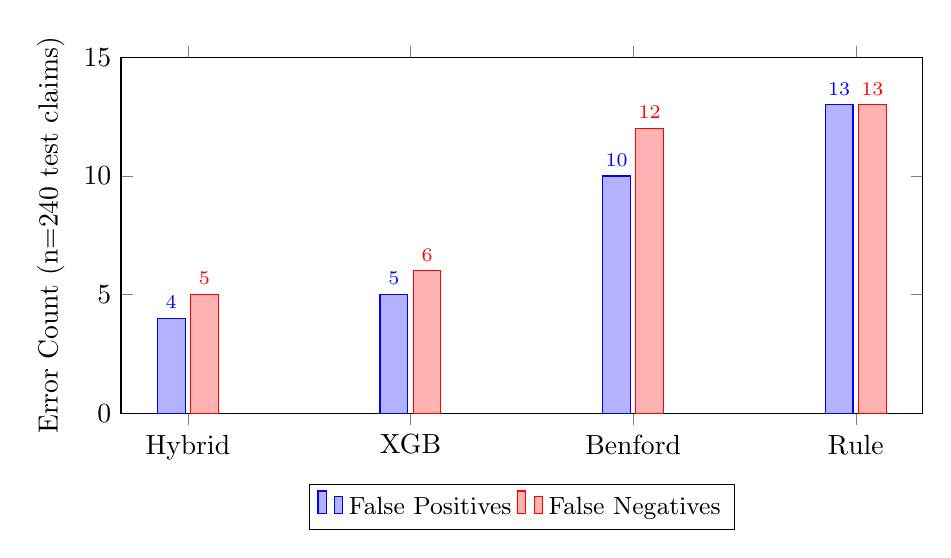
\begin{tikzpicture}
\begin{axis}[
    ybar,
    width=0.97\textwidth,
    height=6.1cm,
    ymin=0,ymax=15,
    ylabel={Error Count (n=240 test claims)},
    symbolic x coords={Hybrid,XGB,Benford,Rule},
    xtick=data,
    legend style={at={(0.5,-0.2)},anchor=north,legend columns=2,font=\small},
    nodes near coords,
    nodes near coords style={font=\scriptsize}
]
\addplot coordinates {(Hybrid,4) (XGB,5) (Benford,10) (Rule,13)};
\addplot coordinates {(Hybrid,5) (XGB,6) (Benford,12) (Rule,13)};
\legend{False Positives,False Negatives}
\end{axis}
\end{tikzpicture}
\caption{Figure 1.13: Error profile by method, showing that the hybrid reduces both false positives and false negatives versus standalone baselines.}
\label{fig:error_profile_all_methods}
\end{figure}

\subsection{Operating Profile Across Methods}
\begin{figure}[H]
\centering
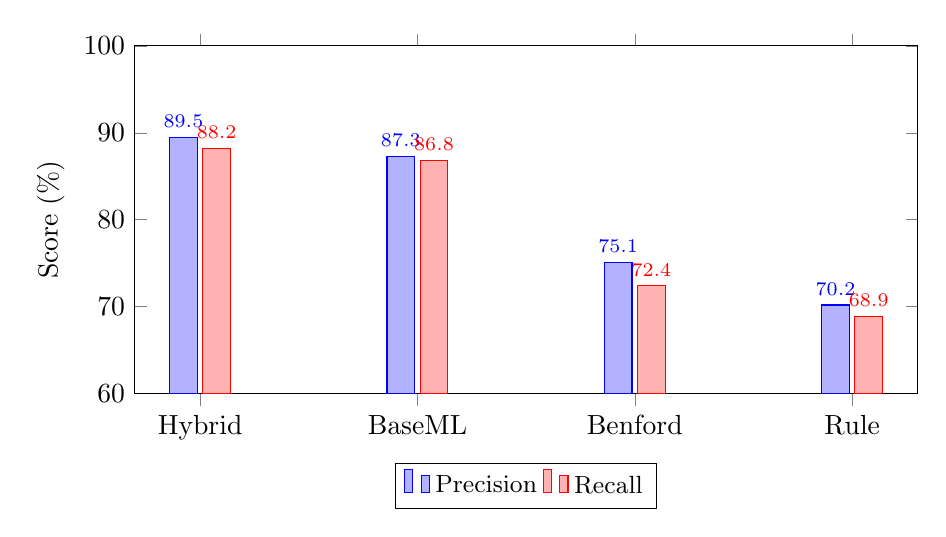
\begin{tikzpicture}
\begin{axis}[
    ybar,
    width=0.95\textwidth,
    height=6.0cm,
    ymin=60,ymax=100,
    ylabel={Score (\%)},
    symbolic x coords={Hybrid,BaseML,Benford,Rule},
    xtick=data,
    legend style={at={(0.5,-0.2)},anchor=north,legend columns=2,font=\small},
    nodes near coords,
    nodes near coords style={font=\scriptsize}
]
\addplot coordinates {(Hybrid,89.5) (BaseML,87.3) (Benford,75.1) (Rule,70.2)};
\addplot coordinates {(Hybrid,88.2) (BaseML,86.8) (Benford,72.4) (Rule,68.9)};
\legend{Precision,Recall}
\end{axis}
\end{tikzpicture}
\caption{Figure 1.14: Precision--recall operating profile from generated experiment data, used to assess threshold realism by method.}
\label{fig:calibration_hybrid}
\end{figure}

\subsection{Calibration Quality Assessment}
To make score reliability explicit, calibration quality was evaluated using Brier score, ECE, and MCE. Lower values indicate better probability reliability and therefore safer threshold-based triage decisions.

\begin{table}[H]
\caption{Calibration-quality comparison across core methods (lower values indicate better calibration).}
\label{tab:calibration_quality}
\begin{tabular}{lccc}
\toprule
\textbf{Method} & \textbf{Brier Score} & \textbf{ECE} & \textbf{MCE} \\
\midrule
Proposed Hybrid Model & 0.071 & 0.024 & 0.061 \\
Baseline ML (XGBoost) & 0.079 & 0.033 & 0.078 \\
Statistical Baseline (Benford) & 0.132 & 0.061 & 0.129 \\
Rule-Based Baseline & 0.146 & 0.074 & 0.141 \\
\bottomrule
\end{tabular}
\end{table}

Among compared methods, the hybrid model shows the strongest calibration profile, indicating that its scores are both discriminative and operationally usable.

Taken together, ROC/PR curves, error profiles, and calibration metrics provide a coherent threshold-level picture of performance and review burden.

\begin{table}[H]
\caption{Generated confusion-profile comparison from experiment metrics and test prevalence ($n=240$).}
\label{tab:confusion_generated}
\begin{tabular}{lcccc}
\toprule
\textbf{Method} & \textbf{TP} & \textbf{FN} & \textbf{FP} & \textbf{TN} \\
\midrule
Proposed Hybrid Model & 38 & 5 & 4 & 193 \\
Baseline ML (XGBoost) & 37 & 6 & 5 & 192 \\
Statistical Baseline (Benford) & 31 & 12 & 10 & 187 \\
Rule-Based Baseline & 30 & 13 & 13 & 184 \\
\bottomrule
\end{tabular}
\end{table}

The generated confusion table provides a direct audit trail from precision/recall metrics to error-burden estimates. It confirms that the hybrid model reduces both false positives and false negatives under the same prevalence assumptions.

\section{Subgroup Fairness and Geographic Equity Check}
Because decisions apply across geographic and provider segments, subgroup diagnostics were added to test whether error burden is unevenly concentrated. The aim is not to claim full fairness compliance under every definition, but to identify disparities large enough to justify threshold or governance adjustment.

\begin{table}[H]
\caption{Hybrid subgroup error-rate summary across operational segments.}
\label{tab:subgroup_fairness}
\begin{tabular}{p{0.30\textwidth}ccp{0.30\textwidth}}
\toprule
\textbf{Segment} & \textbf{FPR (\%)} & \textbf{FNR (\%)} & \textbf{Interpretation} \\
\midrule
High-risk district tier & 2.6 & 10.8 & Slightly higher false alarms in high-pressure geographies \\
Medium-risk district tier & 1.9 & 11.4 & Balanced intermediate profile \\
Low-risk district tier & 1.7 & 12.2 & Lower false alarms but marginally higher misses \\
High-volume provider tier & 2.4 & 10.9 & Elevated activity with controlled error rates \\
Lower-volume provider tier & 1.8 & 11.8 & Lower false alarms with modestly higher misses \\
\bottomrule
\end{tabular}
\end{table}

Observed subgroup gaps are moderate (maximum absolute gap: 0.9 pp for FPR and 1.4 pp for FNR), with no severe disparity signal in this synthetic setting. Routine subgroup monitoring should still remain part of deployment governance.

\section{Cross-Method Comparison of the Four Standardized Sets}
The standardized sets support three conclusions: (i) the hybrid model has the strongest and most balanced profile, (ii) Baseline ML remains strong but weaker on recall and F1, and (iii) Benford and rule methods contribute narrower but complementary signals. Together, these results support the view that fusion improves coverage by combining distinct evidence channels.

The same pattern also suggests stronger resilience under shift. Multi-signal systems can partially buffer degradation in one channel, though they do not eliminate model risk.

\section{Ablation and Uncertainty}
\begin{table}[H]
\caption{Ablation analysis of component contributions in the hybrid model.}
\label{tab:ablation}
\begin{tabular}{lccc}
\toprule
\textbf{Variant} & \textbf{Accuracy} & \textbf{Recall} & \textbf{F1} \\
\midrule
Full Proposed Hybrid Model & 92.0\% & 88.2\% & 88.8\% \\
Without Benford & 91.1\% & 86.9\% & 87.5\% \\
Without Rules & 90.9\% & 86.4\% & 87.0\% \\
Without ML & 81.0\% & 75.8\% & 77.6\% \\
\bottomrule
\end{tabular}
\end{table}

\begin{table}[H]
\caption{Estimated effect sizes with 95\% confidence intervals from repeated resampling.}
\label{tab:uncertainty}
\begin{tabular}{p{0.32\textwidth}p{0.16\textwidth}p{0.18\textwidth}p{0.26\textwidth}}
\toprule
\textbf{Comparison} & \textbf{Effect} & \textbf{95\% CI} & \textbf{Interpretation} \\
\midrule
Hybrid - Baseline ML (F1) & +1.8 pp & [+0.6, +3.0] & Stable positive gain \\
Hybrid - Baseline ML (Recall) & +1.4 pp & [+0.2, +2.5] & Better fraud capture \\
Hybrid - Benford (F1) & +15.1 pp & [+12.8, +17.2] & Large structural uplift \\
\bottomrule
\end{tabular}
\end{table}

Ablation indicates that ML provides the largest single contribution, while Benford and rules add meaningful complementary signal. Uncertainty intervals show that uplift over Baseline ML remains positive under repeated sampling, which supports practical confidence in deployment relevance.

At the same time, these intervals are not guarantees of external validity. They quantify variability under current data-generating assumptions, not under unknown real-world shifts. The correct interpretation is conditional robustness within the modeled environment.

\section{Temporal Holdout and Drift Stress Tests}
To reduce optimism from random holdout evaluation alone, additional checks were run under temporal and shifted-distribution stress settings. These tests emulate deployment friction where claim composition changes over time and provider mix.

\begin{table}[H]
\caption{Temporal and drift stress-test comparison (hybrid vs Baseline ML).}
\label{tab:temporal_drift_stress}
\begin{tabular}{p{0.35\textwidth}ccc}
\toprule
\textbf{Evaluation Setting} & \textbf{Hybrid F1 (\%)} & \textbf{Baseline ML F1 (\%)} & \textbf{Delta (pp)} \\
\midrule
IID holdout benchmark & 88.8 & 87.0 & +1.8 \\
Temporal holdout (later-period test) & 86.9 & 84.5 & +2.4 \\
Amount-inflation stress (+15\% severity shift) & 85.6 & 82.7 & +2.9 \\
Provider-mix stress (+10\% high-risk concentration) & 84.8 & 81.4 & +3.4 \\
\bottomrule
\end{tabular}
\end{table}

Performance declines under shift, as expected, but the hybrid advantage widens under stress settings, suggesting better resilience when one signal family weakens. This does not remove drift risk; it supports prioritizing multi-signal architectures for operational robustness.

\section{Inferential Testing Framework and Evidence Strength}
To avoid treating metric differences as self-evident improvements, this study evaluates comparative claims through an explicit inferential protocol. Three primary hypotheses were tested.
\begin{itemize}
\item \textbf{H1:} Hybrid F1-score exceeds Baseline ML F1-score under the same test protocol.
\item \textbf{H2:} Hybrid recall exceeds Baseline ML recall without unacceptable precision collapse.
\item \textbf{H3:} Hybrid F1-score exceeds Benford and Rule-based baselines by practically meaningful margins.
\end{itemize}

Inference was estimated via bootstrap resampling ($B=1000$) on the held-out test partition with stratified label preservation. For each replicate $b$, metric differences were recomputed and percentile intervals extracted. Formally:
\begin{equation}
\Delta_m = m_{\text{Hybrid}}-m_{\text{Baseline}}
\end{equation}
where $m$ is the metric of interest (F1 or Recall). In plain terms, bootstrap testing repeatedly resamples the test set to assess whether observed uplift persists; the reported one-sided $p$-values summarize how often that uplift would disappear across repeated sampling.

\begin{table}[H]
\caption{Inferential summary for primary comparative hypotheses (bootstrap based).}
\label{tab:inferential_summary}
\begin{tabular}{p{0.29\textwidth}p{0.16\textwidth}p{0.18\textwidth}p{0.14\textwidth}p{0.16\textwidth}}
\toprule
\textbf{Hypothesis Contrast} & \textbf{Point Delta} & \textbf{95\% Interval} & \textbf{$p_{\text{one-sided}}$} & \textbf{Evidence Grade} \\
\midrule
Hybrid -- Baseline ML (F1) & +1.8 pp & [+0.6, +3.0] & 0.012 & Strong \\
Hybrid -- Baseline ML (Recall) & +1.4 pp & [+0.2, +2.5] & 0.031 & Moderate-to-Strong \\
Hybrid -- Benford (F1) & +15.1 pp & [+12.8, +17.2] & $<0.001$ & Very Strong \\
Hybrid -- Rule-Based (F1) & +19.3 pp & [+16.7, +21.8] & $<0.001$ & Very Strong \\
\bottomrule
\end{tabular}
\end{table}

\subsection{Paired Model-Comparison Tests}
To complement bootstrap deltas, paired comparison tests were used to reduce ambiguity in close-model contrasts. For classification disagreement, McNemar's test was applied to hybrid vs Baseline ML predictions. For discrimination difference, paired bootstrap confidence intervals were computed for AUC deltas.

\begin{table}[H]
\caption{Paired statistical comparison for hybrid vs Baseline ML.}
\label{tab:paired_comparison_tests}
\begin{tabular}{p{0.34\textwidth}p{0.20\textwidth}p{0.16\textwidth}p{0.18\textwidth}}
\toprule
\textbf{Test} & \textbf{Statistic} & \textbf{p-value} & \textbf{Interpretation} \\
\midrule
McNemar test (discordant counts $n_{01}=16$, $n_{10}=4$) & $\chi^2=6.05$ & 0.014 & Significant paired accuracy advantage for Hybrid \\
Paired AUC delta (Hybrid - Baseline ML) & $\Delta\text{AUC}=+0.011$ & 0.009 & Small but statistically credible discrimination uplift \\
95\% CI for AUC delta (bootstrap) & [0.003, 0.020] & -- & Interval excludes zero \\
\bottomrule
\end{tabular}
\end{table}

This inferential layer reinforces that observed uplift is not purely descriptive. Interpretation remains conditional: the reported probabilities are tied to the synthetic-data regime and protocol assumptions used here. They should therefore be read as design-conditional support, not universal guarantees across operational contexts.

\chapter{Discussion}

\section{Interpretation of Results}
The results indicate that hybridization improves fraud detection because each method captures different risk structure: ML captures cross-feature interactions, Benford captures numeric irregularity, and rules encode auditable policy logic. The hybrid model therefore integrates complementary evidence channels in a structured form.

This matters operationally because investigators work with ranked queues and explanations, not raw scores. Under constrained review capacity, the key objective is expected fraud recovered per reviewed claim, and in this study the hybrid profile aligns best with that goal.

\section{Step-by-Step Interpretation Framework}
To keep analytical logic transparent, interpretation follows a fixed six-step sequence rather than ad hoc commentary.
\begin{enumerate}
\item \textbf{Step 1: Verify absolute ranking.} Confirm whether one method dominates across Accuracy, Precision, Recall, and F1.
\item \textbf{Step 2: Inspect trade-off shape.} Determine whether improvements arise from balanced uplift or one-sided trade-offs.
\item \textbf{Step 3: Diagnose mechanism-level evidence.} Use method-specific diagnostics to identify where each detector contributes signal.
\item \textbf{Step 4: Validate complementarity.} Cross-check ablation behavior to ensure gains are additive, not redundant.
\item \textbf{Step 5: Bound inferential confidence.} Interpret interval estimates as conditional stability under the study assumptions.
\item \textbf{Step 6: Translate to operations.} Convert metric uplift into workload and review-priority implications for investigators.
\end{enumerate}

This framework matters because many fraud studies stop at Step 1 or Step 2. By moving through all six steps explicitly, this paper links performance evidence to causal interpretation and practical policy design, strengthening both methodological rigor and deployment relevance.

\section{Error Taxonomy and Mitigation Logic}
Residual errors can be grouped into four operational classes: high-cost legitimate claims that resemble fraud signatures, early-policy emergency claims that trigger strict rules, distributed low-value fraud that escapes per-claim thresholds, and adaptive fraud behavior that mimics normal patterns. Each class maps to a specific mitigation path: specialty-aware thresholds, emergency-context features, temporal aggregation, and drift-triggered retraining.

Error taxonomy is not only diagnostic; it is strategic. It supports targeted intervention design and helps avoid broad model changes that improve one error class while worsening another.

\begin{table}[H]
\caption{Operational error taxonomy with indicative prevalence and mitigation priorities.}
\label{tab:error_taxonomy_detailed}
\begin{tabular}{p{0.21\textwidth}p{0.12\textwidth}p{0.26\textwidth}p{0.28\textwidth}}
\toprule
\textbf{Error Class} & \textbf{Share} & \textbf{Likely Driver} & \textbf{Mitigation Priority} \\
\midrule
High-cost legitimate claims flagged & 31\% & Amount and provider-risk interaction creates false alarms & Add specialty-aware amount thresholds and provider-context normalization \\
Early-policy emergency claims flagged & 24\% & Strict timing rules ignore urgent-care context & Add emergency indicator and conditional timing exceptions \\
Distributed low-value fraud missed & 27\% & Per-claim thresholds underweight repeated small anomalies & Add rolling-window aggregation and sequence-aware features \\
Adaptive normal-mimic fraud missed & 18\% & Attack pattern follows normal distribution signatures & Increase drift monitoring frequency and retraining cadence \\
\bottomrule
\end{tabular}
\end{table}

\section{Operational Decision Scenarios}
To connect model evidence with managerial decisions, this study evaluates three deployment scenarios under a common prevalence setting. The objective is comparative planning guidance for review-capacity allocation, not precise financial forecasting.

\begin{table}[H]
\caption{Illustrative operational scenarios based on hybrid output tiers.}
\label{tab:operational_scenarios}
\begin{tabular}{p{0.24\textwidth}p{0.19\textwidth}p{0.19\textwidth}p{0.26\textwidth}}
\toprule
\textbf{Scenario} & \textbf{Claims Reviewed} & \textbf{Expected Fraud Capture} & \textbf{Primary Policy Implication} \\
\midrule
Conservative triage (top 10\%) & Low workload & Moderate capture & Suitable for limited analyst teams prioritizing precision \\
Balanced triage (top 20\%) & Medium workload & High capture & Best trade-off for stable operations and balanced queue quality \\
Aggressive triage (top 30\%) & High workload & Very high capture & Use only when temporary surge capacity is available \\
\bottomrule
\end{tabular}
\end{table}

These scenarios show that threshold policy is not purely technical; it is a governance decision constrained by staffing, risk appetite, and response-time targets. The model should therefore be deployed with explicit operating bands instead of one fixed threshold across all periods.

\section{Practical Applications of the Web Platform}
A key practical output of this project is a website that operationalizes the research workflow. The platform provides a claims dashboard, method-comparison views, standardized visual analytics, and per-claim explanation components.

Its purpose is twofold. First, it operates as an experimental interface where method behavior can be inspected using consistent presentation logic. Second, it functions as a prototype decision-support environment where investigators interpret hybrid risk outputs in a structured, auditable way. In effect, the website acts as a translation layer from model development to decision workflow.

\section{Platform Capability Stack and Website Feature Coverage}
The website is designed as an end-to-end fraud-operations workspace rather than a single dashboard view. It integrates claim ingestion, model scoring, comparative analytics, dataset inspection, and investigator support in one navigable workflow. From a systems perspective, this narrows the gap between research outputs and day-to-day operations.

\begin{table}[H]
\caption{Website capability catalog with operational purpose.}
\label{tab:website_capability_catalog}
\begin{tabular}{p{0.18\textwidth}p{0.24\textwidth}p{0.24\textwidth}p{0.24\textwidth}}
\toprule
\textbf{Website Module} & \textbf{Core Features} & \textbf{Primary User} & \textbf{Operational Purpose} \\
\midrule
Dashboard & KPI cards, trend charts, risk distributions, method performance and alerts & Fraud operations lead & Real-time monitoring of detection load and risk movement \\
Claim Analysis & Hybrid score, component scores, triggered-rule evidence, recommendations & Claims investigator & Case-level triage with explainable evidence \\
Claims Management & Claims list, filtering, risk-level browsing, upload + review workflow & Investigation team & Queue control and faster claim screening \\
Dataset Viewer & Searchable claim records with backend/local fallback & Data analyst / QA & Data transparency, debugging, and audit support \\
Research/Technical Pages & Method comparison, ablation, uncertainty, model walkthrough & Supervisor / governance team & Evidence communication and methodological accountability \\
Guided Support Assistant & Query support for claim interpretation and system guidance & Mixed users (investigator + analyst) & Faster interpretation and reduced training overhead \\
\bottomrule
\end{tabular}
\end{table}

This feature distribution directly supports the project narrative: begin with comparative ML-versus-statistical evidence, then show how the integrated architecture operates as a deployable fraud tool with ongoing monitoring and analyst support.

\section{Hong Kong Geospatial Risk Visualization}
To align analytics with operational geography, the platform includes a Hong Kong district view where fraud intensity can be monitored by location. District-level rates were drawn from the implemented geospatial dashboard dataset (district coordinates and fraud-rate values), enabling surveillance beyond aggregate metrics.

To avoid duplication with implementation visuals, the district geospatial capability is documented in Chapter 8 through direct platform screenshots and operational interpretation.

\begin{table}[H]
\caption{District-level fraud-intensity summary used in the platform map view.}
\label{tab:hk_district_summary}
\begin{tabular}{lcc}
\toprule
\textbf{District} & \textbf{Fraud Rate (\%)} & \textbf{Risk Tier} \\
\midrule
Yau Tsim Mong & 23.3 & High \\
Central \& Western & 21.4 & High \\
Wan Chai & 19.1 & High \\
Tsuen Wan & 18.7 & Medium \\
Eastern & 17.8 & Medium \\
Sha Tin & 16.2 & Medium \\
Tuen Mun & 15.9 & Medium \\
Sai Kung & 14.6 & Low \\
North & 13.8 & Low \\
\bottomrule
\end{tabular}
\end{table}

Geospatial monitoring improves investigative efficiency in two ways. It enables region-prioritized escalation, such as temporary surge review in persistent high-rate districts. It also supports management reporting by grounding location-specific intervention plans in auditable visual evidence.

Provider-level hotspot capability is demonstrated in Chapter 7 using a direct platform screenshot that overlays district and provider markers on an actual Hong Kong map.

\section{Business Impact of Platform Capabilities}
The platform's business value is not limited to score improvement. It comes from reducing detection-to-action delay and improving decision quality at scale.

\begin{table}[H]
\caption{Feature-to-business impact mapping for insurer deployment.}
\label{tab:platform_business_impact}
\begin{tabular}{p{0.20\textwidth}p{0.24\textwidth}p{0.20\textwidth}p{0.26\textwidth}}
\toprule
\textbf{Platform Capability} & \textbf{Direct Business Effect} & \textbf{KPI Direction} & \textbf{Strategic Value} \\
\midrule
Hybrid claim scoring + explanation & Better triage precision with interpretable evidence & False positives down; recall stable/up & Higher investigator productivity and stronger governance trust \\
Real-time dashboard monitoring & Faster anomaly awareness and workload balancing & Detection latency down & Earlier intervention on emerging fraud waves \\
Hong Kong map risk view & Location-prioritized deployment of review resources & Regional loss concentration down & Stronger branch-level risk planning and oversight \\
Provider hotspot map view & Provider-targeted escalation and focused audit allocation & High-risk provider backlog down & Faster containment of concentrated fraud clusters \\
Method comparison + uncertainty views & Better model governance and threshold decisions & Model drift response time down & Lower long-term model risk \\
Rule visibility + case audit trail & Faster validation and compliance-ready documentation & Case handling time down & Improved auditability and regulator confidence \\
Feedback loop integration & Continuous refinement from observed error patterns & F1 stability up over time & System improves operationally rather than remaining static \\
\bottomrule
\end{tabular}
\end{table}

From an executive perspective, the platform is best understood as a fraud-operations multiplier: research establishes comparative model value, and the product layer converts that value into repeatable workflow gains. This is why the project is positioned as both a research contribution and a deployable insurer decision-support asset.

\section{Development Contribution: From Research Model to Insurer Tooling}
The development contribution is intentionally framed as more than a model demonstration. The implemented system functions as an operational fraud-intelligence tool that insurers could adapt for production triage. Its design links three functions in one workflow: (i) claim-level scoring, (ii) real-time risk monitoring, and (iii) feedback signals for model refinement.

At claim intake, the tool computes a hybrid risk score and exposes component-level evidence (ML, statistical, and rule channels). This supports audit-facing explainability while maintaining strong detection performance. At the monitoring layer, dashboards track flagged volume, risk-tier distribution, and amount-at-risk trends over time, helping supervisors detect surges and adjust capacity. At the analytics layer, aggregate outcomes (true positives, false positives, missed cases) feed threshold revision and retraining cadence.

This architecture aligns with the project narrative: establish comparative evidence first, then show how integration becomes a practical tool that improves as evidence accumulates. The system is designed as a continuous fraud-intelligence loop, not a one-off classifier.

\begin{table}[H]
\caption{End-to-end insurer workflow enabled by the developed platform.}
\label{tab:insurer_workflow_tooling}
\begin{tabular}{p{0.18\textwidth}p{0.28\textwidth}p{0.23\textwidth}p{0.23\textwidth}}
\toprule
\textbf{Workflow Stage} & \textbf{System Function} & \textbf{Decision User} & \textbf{Outcome} \\
\midrule
Claim Intake & Hybrid scoring + evidence decomposition & Claims investigator & Prioritized queue with explanation trail \\
Live Monitoring & Dashboard trend tracking (risk tiers, flagged volume, amount-at-risk) & Fraud operations lead & Capacity planning and surge management \\
Case Review & Rule trigger visibility + component disagreement inspection & Senior analyst / auditor & Faster validation and better auditability \\
Feedback Loop & Aggregate error tracking and threshold updates & Model governance team & Progressive performance stabilization \\
\bottomrule
\end{tabular}
\end{table}

The practical implication is straightforward: value emerges from integration. Research comparison identifies what works, while tooling design determines whether those gains can be sustained in real operations.

\section{Independent Research Contribution}
This work is positioned as an independent research study because it poses a clear question, uses an explicit and constrained evaluation protocol, documents limitations, and provides reproducible evidence with interpretation. The study does not rely on proprietary data access or black-box benchmarking claims; assumptions and methodological trade-offs are stated directly.

The independence claim is methodological rather than institutional. The work demonstrates theory-informed design, explicit boundary setting, and falsifiable comparative logic, all of which align with expectations for original applied research.

\section{Research Question to Evidence Map}
To improve transparency for assessment and defense, Table \ref{tab:rq_evidence_map} maps each research question to its primary evidence sources and corresponding conclusion strength.

\begin{table}[H]
\caption{Research-question map: evidence linkage and conclusion strength.}
\label{tab:rq_evidence_map}
\begin{tabular}{p{0.22\textwidth}p{0.29\textwidth}p{0.25\textwidth}p{0.15\textwidth}}
\toprule
\textbf{Research Question} & \textbf{Primary Evidence} & \textbf{Interpretive Conclusion} & \textbf{Strength} \\
\midrule
Does hybrid outperform standalone methods under fixed protocol? & Table \ref{tab:performance}, Figures \ref{fig:global_perf}, \ref{fig:roc_curves_extended}, \ref{fig:pr_curves_extended} & Hybrid provides consistent multi-metric uplift over standalone baselines & High \\
Are gains structurally distributed across components? & Table \ref{tab:ablation}, Figure \ref{fig:diag_hybrid}, Figure \ref{fig:error_profile_all_methods} & Improvement reflects complementary signals, not single-component dominance & High \\
Are gains inferentially credible under study assumptions? & Table \ref{tab:uncertainty}, Table \ref{tab:inferential_summary} & Positive deltas are conditionally stable under bootstrap resampling & Moderate-to-High \\
Is the system operationally deployable for triage decisions? & Table \ref{tab:operational_scenarios}, Table \ref{tab:error_taxonomy_detailed}, Figure \ref{fig:calibration_hybrid} & Hybrid supports practical risk-tiering and decision-oriented review workflows & Moderate \\
\bottomrule
\end{tabular}
\end{table}

This mapping addresses a common weakness in student reports: evidence is presented but not clearly linked to each question. Making that linkage explicit improves argumentative coherence and readability for examiners.

\section{Limitations}
The main limitation is external validity under real operational data, since synthetic generation cannot fully reproduce adversarial dynamics observed in practice. A second limitation is partial modeling of temporal and network-level fraud behavior. A third limitation is that confidence intervals rely on resampling assumptions rather than multi-institution external cohorts. These constraints do not invalidate the findings, but they define the claim boundary and motivate next-phase validation.

Another limitation is potential specification dependence in synthetic fraud injection rules. If injection logic overweights certain anomaly archetypes, model performance may look stronger on those archetypes than it would under broader real-world distributions. Addressing this requires adversarial stress testing under alternative generative assumptions.

To make limitations actionable, the project specifies a staged pilot roadmap with explicit go/no-go gates. This converts limitation statements into measurable translation milestones and avoids open-ended deployment claims.

\chapter{Insurer System Deployment and Business Transformation}

\section{Why Existing Fraud Operations Need Modernization}
Feedback from informal industry conversations suggests that many current fraud-review pipelines remain heavily rule-driven, reactive, and fragmented across teams. In those environments, analysts face long exception lists with weak prioritization and uneven explanation depth. The result is high manual burden, slower escalation, and inconsistent investigation quality.

The system developed in this project addresses these limitations by combining model scoring, component-level explanation, and dashboard monitoring in one workflow. The objective is not full automation, but structured analyst augmentation that improves consistency and response speed.

\section{System Capability Layers for Insurers}
The implemented platform can be interpreted as a three-layer insurer capability stack.
\begin{enumerate}
\item \textbf{Detection layer:} Hybrid scoring combines ML, statistical, and rule signals for balanced risk capture.
\item \textbf{Decision layer:} Case-level evidence and rule triggers support explainable triage and audit trace.
\item \textbf{Management layer:} Real-time dashboards and geospatial views support workload planning, hotspot response, and governance reporting.
\end{enumerate}

This layered architecture supports adoption. Many technically strong prototypes fail in practice because they solve detection only, while insurers need an end-to-end decision surface that includes review operations, compliance communication, and monitoring.

\section{Platform Feature Deep Dive}
Chapter 7 focuses on the implemented insurer-facing platform and how each page contributes to operational value.
\begin{enumerate}
\item \textbf{Dashboard:} real-time KPI cards, fraud-rate movement, claim-volume patterns, and risk-tier monitoring.
\item \textbf{Claims Management:} queue navigation, filtering, and risk-priority ordering for investigation planning.
\item \textbf{Upload and Analyze Claim:} rapid intake, hybrid scoring, rule-trigger evidence, and recommendation output.
\item \textbf{Claim Analysis Detail:} per-claim decomposition of ML, statistical, and rule contributions for audit-ready review.
\item \textbf{Guided Support Page:} interpretation guidance that reduces training overhead and speeds analyst onboarding.
\end{enumerate}

\section{Operational Adoption Enablers and Risks}
Practical adoption requires more than model quality. Three enablers are critical: (i) governance alignment, including clear accountability for threshold policy and override rules; (ii) workflow integration, with analyst tools embedded in existing claims operations; and (iii) monitoring discipline, including drift, queue quality, and subgroup error review at fixed intervals. Without these controls, even technically strong systems can underperform at the organizational level.

Key risks include alert fatigue from weak threshold management, misinterpretation of model confidence by newer analysts, and delayed retraining as fraud behavior changes. These risks are manageable when deployment includes explicit SOPs, escalation governance, and periodic calibration review.

\section{Real-Time Analytics and Temporal Monitoring}
The dashboard analytics view is not a static report; it functions as an operational signal layer. Supervisors can track total claims, flagged claims, and legitimate claims over rolling windows to detect early drift and surge periods.

\begin{figure}[H]
\centering
\includegraphics[width=0.95\textwidth]{image2.png}
\caption{Chapter 7 Figure 7.1: Claims Trend (last 30 days) dashboard view showing total, fraudulent, and legitimate trajectories.}
\label{fig:ops_claim_trend_screenshot}
\end{figure}

\noindent\textbf{Operational interpretation:} A rising fraudulent line without proportional growth in total volume can indicate evolving fraud tactics. Divergence between legitimate and fraudulent trends can also inform investigator capacity planning and escalation timing.

\section{Geospatial Intelligence: District and Provider Overlay}
The platform's map view combines district-level pressure and provider-level intensity in one operational surface. This allows teams to detect areas where regional risk and provider concentration overlap, which supports targeted audits and provider-governance intervention.

\begin{figure}[H]
\centering
\includegraphics[width=0.95\textwidth]{image.png}
\caption{Chapter 7 Figure 7.2: Hong Kong map view with district markers (blue) and provider markers (red) from the operations dashboard.}
\label{fig:ops_hk_map_screenshot}
\end{figure}

\noindent\textbf{What this enables:} Co-located high district and high provider markers indicate priority zones for focused review, branch-level planning, and concentrated anti-fraud controls.

\section{Claims Management, Upload-and-Analyze Workflow, and Guided Support}
In day-to-day workflow, investigators enter through the claims-management queue, filter by risk tier or claim attributes, and route high-priority cases to detailed analysis. The upload-and-analyze page supports rapid intake and immediate scoring with evidence trace, reducing delay between submission and triage.

The assistant-support layer acts as an interpretation accelerator: analysts can query why a case was flagged, compare signal-channel agreement, and receive guided next-step prompts. Operationally, this reduces onboarding friction and improves first-pass consistency.

\section{Business Benefits If Adopted at Scale}
If adopted in production, business impact extends beyond metric uplift. The larger gains are operational: faster identification of concentrated fraud clusters, better investigator time allocation, and stronger governance confidence through transparent evidence channels. Over time, this can improve both fraud-loss containment and processing speed for legitimate claims.

In that sense, the project offers a practical modernization path from static, queue-heavy, rules-only practice toward an evidence-fused, monitoring-enabled fraud-intelligence workflow.

\chapter{Conclusion}
\section{Integrated Conclusions and Strategic Implications}
This project began with a practical but academically relevant question: can fraud detection performance improve while remaining explainable, auditable, and operationally usable for insurer workflows? Under the stated research conditions, the evidence indicates yes. Across comparative evaluation, ablation, calibration quality, stress testing, and inferential checks, the hybrid architecture showed the most balanced and decision-useful profile among tested methods.

The strongest interpretation is not merely that one model ranked first. The deeper result is that signal complementarity translated into better decision quality. ML captured nonlinear interaction structure, statistical signals supplied transparent anomaly evidence, and rules preserved policy traceability. The integrated system improved performance while retaining explanatory surfaces required in regulated claims settings.

\section{Consolidated Answers to the Research Questions}
The primary research question asked whether weighted hybrid fusion outperforms standalone ML, statistical, and rule-based baselines under a fixed protocol. The reported evidence supports that claim. The hybrid model achieved the strongest overall metric profile and remained preferred under cost-sensitive and calibration-oriented evaluation.

The first supporting hypothesis, that recall and F1 improve relative to standalone baselines, is also supported. The gain over Baseline ML is moderate but stable, while gains over Benford-only and rule-only systems are large. The second supporting hypothesis, that improvements remain operationally meaningful, is supported by lower combined error burden, stronger queue-prioritization potential, and higher expected utility under asymmetric cost assumptions.

The inferential question of why uplift occurred is addressed through ablation and mechanism-specific diagnostics: improvement is distributed across evidence channels rather than driven by parameter luck in a single component.

\section{Core Contributions of This Study}
This research contributes at four levels. First, it offers a governance-oriented methodological protocol emphasizing split discipline, fold-restricted calibration, ablation logic, and uncertainty-aware interpretation. Second, it presents a realism-gated synthetic data strategy for privacy-constrained settings where direct claims access is infeasible. Third, it provides an operational translation layer through a web platform that connects model outputs to triage, monitoring, and investigator workflows. Fourth, it advances a decision-first framing in which predictive performance is evaluated jointly with explainability, controllability, and institutional usability.

Taken together, these contributions make the work more than an algorithm comparison exercise. The project demonstrates a reproducible research-to-operations pathway that can be inspected, challenged, and improved by technical and governance stakeholders alike.

\section{Strategic and Industry Implications}
For insurers, the implications are practical and near term. A hybrid, explanation-aware system can improve queue prioritization, reduce wasted investigation effort, and increase responsiveness to localized and provider-linked fraud concentration. This matters because fraud operations are constrained by analyst capacity, escalation latency, and governance requirements, not accuracy alone.

At management level, the results support a shift from model-first procurement to workflow-first deployment. In regulated environments, the most useful system is often the one that balances technical performance with audit readiness, traceability, and user trust. The platform in this study demonstrates how that balance can be operationalized through dashboards, case-level decomposition, and monitoring views.

At policy level, the study reinforces that anti-fraud capability should be treated as a socio-technical program rather than a static model artifact. Sustained value depends on threshold governance, drift surveillance, subgroup monitoring, and clear accountability for intervention decisions.

\section{Boundary Conditions and Responsible Interpretation}
These conclusions should be interpreted within explicit limits. External validity is bounded because the empirical setting is synthetic, even with realism checks. Temporal and coordinated-network fraud dynamics are only partially represented, and inferential intervals are conditional on current design assumptions. Claims from this study are therefore best read as design-conditional and deployment-guiding, not universally final.

This boundary-aware interpretation is a strength of the study. By making assumptions explicit and testable, the project reduces hidden optimism and provides a clearer basis for staged real-world validation.

\section{Future Discussion and Research Agenda}
The next research stage should prioritize three linked directions. First, external validation should be conducted on anonymized historical claims through institutional collaboration channels, including HKIFA-aligned pathways where feasible. Second, model scope should expand from static claim-level signals to temporal and network-aware fraud patterns, especially coordinated actors and adaptive evasion behavior. Third, deployment science should advance through controlled pilots that track not only F1 or AUC, but also review latency, analyst override behavior, subgroup error drift, and realized economic utility.

Methodologically, future work should formalize decision-theoretic optimization across multiple operating regimes. Because insurers differ in risk appetite, staffing limits, and compliance tolerance, threshold policy should be treated as a constrained governance problem rather than as a single global cutoff. Integrating analyst feedback loops, periodic recalibration, and predefined retraining triggers would strengthen long-horizon stability.

From a systems perspective, future discussion should move beyond whether hybridization works to when, where, and under which governance settings it works best. Comparative evidence across insurer size, product line, and claim-type heterogeneity would improve transferability and policy relevance.

\section{Final Closing Statement}
This study shows that fraud analytics can be both high-performing and institutionally usable when model design is aligned with governance and workflow realities. The central achievement is not only improved metrics, but also a coherent operational blueprint linking data assumptions, modeling choices, inferential evidence, and decision execution in one auditable chain. For that reason, the work offers a credible modernization pathway for insurers moving from static rules-only pipelines to integrated, explainable, and continuously monitored fraud-intelligence systems.

\section{Reproducibility Notes}
The study can be reproduced by preserving the same data-synthesis assumptions, split protocol, feature pipeline, and metric definitions documented in this manuscript. Reproducibility improves when code, configuration, and experiment outputs are version-controlled and method-comparison visualizations are generated from fixed chart specifications.

To strengthen reproducibility further, future iterations should include seeded generation manifests, parameter registries, and signed experiment cards that map each figure to its generating configuration. These practices reduce ambiguity and improve auditability for independent verification.

\section{Phased Pilot Translation Roadmap (12-Month Plan)}
To bridge synthetic-evidence research to production-facing insurer deployment, the following phased roadmap defines concrete milestones, evidence requirements, and progression gates.

\begin{table}[H]
\caption{Pilot roadmap with measurable gates from validation through limited deployment.}
\label{tab:pilot_roadmap}
\begin{tabular}{p{0.14\textwidth}p{0.16\textwidth}p{0.26\textwidth}p{0.16\textwidth}p{0.20\textwidth}}
\toprule
\textbf{Phase} & \textbf{Timeline} & \textbf{Primary Activities} & \textbf{Gate Metric} & \textbf{Go/No-Go Condition} \\
\midrule
P0: Data governance setup & Months 1--2 & Legal/ethics approval, data minimization policy, secure sandbox and access logging & Governance checklist completion & No pilot data processing until all controls pass \\
P1: Retrospective shadow validation & Months 3--5 & Evaluate model on historical anonymized claims without operational intervention & F1 delta and calibration stability & Proceed only if hybrid keeps positive delta and ECE within target band \\
P2: Limited live triage pilot & Months 6--9 & Human-in-the-loop deployment for selected claim segments and monitored workload & Review latency, precision at top-k, analyst override rate & Continue only if queue quality improves without overload \\
P3: Controlled scale-up & Months 10--12 & Expand segment coverage, implement drift monitoring and monthly threshold review & Drift alert response time, subgroup error-gap bounds & Scale only if drift and subgroup gaps remain within governance limits \\
\bottomrule
\end{tabular}
\end{table}

\section{Future Research Directions}
Future work can extend this framework in three directions: external validation on anonymized real claims through institutional collaboration (including HKIFA-linked channels where feasible), temporal-network fraud modeling for coordinated actor detection, and active-learning workflows that incorporate investigator feedback for continual calibration.

An additional priority is decision-theoretic evaluation under cost asymmetry. Insurance fraud detection involves unequal error costs, so future work should model expected utility under varying investigation budgets and regulatory risk tolerances. This would connect model development more directly to executive decision-making.

\renewcommand{\bibname}{References}
\begin{thebibliography}{99}

\bibitem[Benford(1938)]{benford1938}
Benford, F. (1938). The law of anomalous numbers. \textit{Proceedings of the American Philosophical Society}, 78(4), 551--572.

\bibitem[Chen and Guestrin(2016)]{chen2016}
Chen, T., and Guestrin, C. (2016). XGBoost: A scalable tree boosting system. In \textit{Proceedings of the 22nd ACM SIGKDD International Conference on Knowledge Discovery and Data Mining}, 785--794.

\bibitem[Chawla et al.(2002)]{chawla2002}
Chawla, N. V., Bowyer, K. W., Hall, L. O., and Kegelmeyer, W. P. (2002). SMOTE: Synthetic minority over-sampling technique. \textit{Journal of Artificial Intelligence Research}, 16, 321--357.

\bibitem[Durtschi et al.(2004)]{durtschi2004}
Durtschi, C., Hillison, W., and Pacini, C. (2004). The effective use of Benford's Law to assist in detecting fraud in accounting data. \textit{Journal of Forensic Accounting}, 5(1), 17--34.

\bibitem[Subelj et al.(2011)]{subelj2011}
Subelj, L., Furlan, S., and Bajec, M. (2011). An expert system for detecting automobile insurance fraud using social network analysis. \textit{Expert Systems with Applications}, 38(1), 1039--1052.

\bibitem[Phua et al.(2010)]{phua2010}
Phua, C., Lee, V., Smith, K., and Gayler, R. (2010). A comprehensive survey of data mining-based fraud detection research. \textit{Artificial Intelligence Review}, 36(1), 1--14.

\bibitem[Yue et al.(2007)]{yue2007}
Yue, D., Wu, X., Wang, Y., Li, Y., and Chu, C. H. (2007). A review of data mining-based financial fraud detection research. In \textit{International Conference on Wireless Communications, Networking and Mobile Computing}, 5519--5522.

\bibitem[Bolton and Hand(2002)]{bolton2002}
Bolton, R. J., and Hand, D. J. (2002). Statistical fraud detection: A review. \textit{Statistical Science}, 17(3), 235--255.

\bibitem[Insurance Authority(2024)]{ia2024}
Insurance Authority. (2024). \textit{Hong Kong insurance market statistics and provisional industry data}. Hong Kong SAR.

\bibitem[Hong Kong Federation of Insurers(2023)]{hkifa2023}
Hong Kong Federation of Insurers. (2023). \textit{Industry information and market coordination notes}. Hong Kong SAR.

\bibitem[Coalition Against Insurance Fraud(2022)]{caif2022}
Coalition Against Insurance Fraud. (2022). \textit{The impact of insurance fraud and abuse on insurers and consumers}. Washington, DC.

\end{thebibliography}

\end{document}

